% !TeX program = pdflatex
% Computer Physics Communications -- regular article draft.
% Build:  latexmk -pdf main.tex      (or: pdflatex main; pdflatex main)
\documentclass[preprint,12pt,number]{elsarticle}

\usepackage[T1]{fontenc}
\usepackage[utf8]{inputenc}
\usepackage{amsmath,amssymb,amsthm}
\usepackage{graphicx}
\usepackage{booktabs}
\usepackage{multirow}
\usepackage{tikz}
\usetikzlibrary{arrows.meta,positioning,fit,backgrounds,calc}
\usepackage{pgfplots}
\pgfplotsset{compat=1.17}
\usepackage{subcaption}
\usepackage{hyperref}
\usepackage{xcolor}
\usepackage{microtype}

\graphicspath{{figures/}}
\newcommand{\Hh}{H_h}
\newcommand{\norm}[1]{\lVert #1\rVert}
\newcommand{\abs}[1]{\lvert #1\rvert}
\newcommand{\R}{\mathbb{R}}
\newcommand{\spec}{\sigma}

\newtheorem{theorem}{Theorem}
\newtheorem{lemma}{Lemma}
\newtheorem{corollary}{Corollary}
\newtheorem{definition}{Definition}
\newtheorem{remark}{Remark}

% CPC program-summary block (elsarticle defines no environment for it).
\newenvironment{programsummary}
  {\par\medskip\noindent\rule{\linewidth}{0.5pt}\par\vspace{2pt}
   \noindent\textbf{Program summary}\par\nopagebreak\vspace{2pt}\footnotesize}
  {\par\nopagebreak[4]\vspace{2pt}\noindent\rule{\linewidth}{0.5pt}\par\medskip}

\journal{Computer Physics Communications}

\begin{document}

\begin{frontmatter}

\title{Certifying neural eigenpairs and degenerate eigenspaces of the Schr\"odinger
equation: a self-verifying \emph{a posteriori} protocol and its implementation}

\author[inst1]{Chunyang Chen\fnref{fn1}}
\author[inst1]{Yuhao Peng\fnref{fn1}\corref{cor1}}
\ead{pngyuo@cug.edu.cn}
\cortext[cor1]{Corresponding author.}
\fntext[fn1]{These authors contributed equally to this work.}
\affiliation[inst1]{organization={School of Mathematics and Physics,
China University of Geosciences (Wuhan)}, city={Wuhan}, postcode={430074},
country={China}}

\begin{abstract}
Neural solvers of the stationary Schr\"odinger equation are evaluated against
a reference solution that new problems lack. We present a computable
\emph{a posteriori} certificate for neural eigenpairs of the discretized
operator: from an approximate eigenfunction it returns a two-sided eigenvalue
enclosure, a bound on the angle to the true eigenfunction, and a verified
state index, using only the approximation itself. The hypotheses of the
Temple and Davis--Kahan bounds are \emph{verified} rather than assumed, by
counting the spectrum below a shift with Sturm sequences in one dimension and
with the Sylvester inertia of a sparse LU factorization in two; the
one-dimensional count, and the two-dimensional one for separable potentials,
are re-derived in directed rounding, hence theorems about the stored matrix.
A degenerate level has no single eigenfunction to certify, so we extend the
construction to invariant subspaces: the multiplicity is \emph{measured},
cluster eigenvalues are bracketed, and a principal-angle bound certifies the
subspace spanned by several network outputs. On six potentials, all $39$
enclosures contain an independently computed discrete eigenvalue; a
degenerate state with residual $4\times10^{-12}$ is refused individually and
certified as a two-dimensional subspace; independently trained pairs that
span it are separated from collapsed ones. A variational bound on the
interpolant carries one side of the guarantee to the continuous operator.
\end{abstract}

\begin{keyword}
Schr\"odinger equation \sep neural network eigen solver \sep a posteriori error
bound \sep Temple bound \sep Sylvester inertia \sep invariant subspaces \sep
verification
\end{keyword}

\end{frontmatter}

\begin{programsummary}
\noindent\textbf{Program title:} \texttt{nn-schrodinger-certify}\\
\textbf{CPC Library link to program files:} (to be added by Technical Editor)\\
\textbf{Developer's repository link:}\\
\url{https://github.com/YuhaoPeng1103/PINN_equation}\\
\textbf{Licensing provisions:} MIT license (MIT)\\
\textbf{Programming language:} Python 3.11 (NumPy, SciPy; PyTorch for
training)\\
\textbf{Supplementary material:} none\\
\textbf{Nature of problem (approx.\ 50--250 words):} Neural solvers of the
stationary Schr\"odinger equation are evaluated against a reference solution
that a new problem does not have. A small residual does not bound the
eigenfunction error, and at a degenerate level no single eigenfunction is
defined, so the usual comparison is ill-posed as well as unavailable: what is
wanted is a statement computable from the approximation alone.\\
\textbf{Solution method (approx.\ 50--250 words):} Given an approximate eigenfunction, or an
$m$-dimensional trial subspace, on a finite-difference grid, the code returns a
two-sided enclosure of the discrete eigenvalue, a bound on the angle to the
exact eigenfunction or invariant subspace, and a verified state index. The
hypotheses of the Kato--Temple and Davis--Kahan bounds are decided by counting
the spectrum with Sturm sequences in one dimension and with the Sylvester
inertia of a no-pivot sparse LU in two, guarded against silent pivoting and
against a resolution floor; the
one-dimensional count, and the two-dimensional one for separable potentials,
are re-derived in directed-rounding interval arithmetic and refuse when a
pivot or a summed pair is unresolved. A variational bound evaluated on the
P1/Q1 interpolant of a sampled eigenfunction bounds the continuous eigenvalue
from above without a reference solution, and a certificate-selected Dirichlet
sine filter and a transport inequality extend the bound to the raw network
output.\\
\textbf{Additional comments including restrictions and unusual features
(approx.\ 50--250 words):} Includes the drivers that regenerate every table
and figure of the article and a 143-test suite. A count costs $0.03$\,s at
$81\times81$ and $0.4$\,ms at $N=2001$, or $5$\,ms in one dimension with
directed rounding; a full certificate costs $0.07$\,s at $N=2001$ and
$0.2$\,s at $81\times81$. Restriction: the operator must be assemblable, so
the high-dimensional regime is out of reach; the anharmonic potential is
counted in guarded floating point because the general two-dimensional
interval count is measured but not used; the resolution floor is a declared
margin, not a theorem.\\
\textbf{References:} none
\end{programsummary}

\section{Introduction}
\label{sec:intro}

Neural representations of quantum wavefunctions are now used both as
variational ans\"atze for many-body problems \citep{carleo2017,hermann2020,pfau2020}
and as mesh-free solvers for the stationary Schr\"odinger equation
\citep{raissi2019,karniadakis2021}. In the second setting a network $\psi_\theta$ is trained so
that $\Hh\psi_\theta\approx E\psi_\theta$ in a discrete $L^2$ sense, and the
paper reports an energy error and a wavefunction overlap against a reference
solution.

This evaluation scheme has a structural weakness. The reference is either an
analytic solution---available only for textbook potentials---or the output of
a classical solver on the same grid. In the second case the comparison
measures agreement between two approximations, not accuracy, and it silently
absorbs the discretization error of the grid into the "method error". More
importantly, in a genuinely new problem there is no reference at all, and the
only quantities available are those the approximation itself provides. A
residual is such a quantity, but making it small is itself delicate---the
gradient pathologies of residual training are well documented
\citep{wang2021}---and even a small residual is not an error: a residual of
$10^{-2}$ may correspond to an energy error of $10^{-6}$ or to a wavefunction
that is entirely the wrong eigenstate. Both directions occur in the runs
reported below. A network whose energy was accurate to seven digits
($|\eta-\lambda_h|=2.6\times10^{-7}$ on the infinite-well grid) carried a
residual of $0.53$, so that the certificate could prove only an angle bound
of $0.56$~rad and an enclosure six orders of magnitude wider than the true
error (Section~\ref{sec:leak-results}). Conversely, a network trained with a
scale-invariant loss returned a field whose residual norm was
$2.9\times10^{-4}$ while its $L^2$ distance from the eigenfunction of unit norm
was $0.99$: the residual had been made small by shrinking the field
(\ref{app:failures}).

The numerical analysis literature solved the corresponding problem for finite
element and spectral methods long ago: eigenvalue enclosures follow from
variational bounds (Weinstein, Kato--Temple, Lehmann--Goerisch) together with
a verified count of the spectrum in an interval \citep{babuska1991,parlett1998},
and eigenvector bounds follow from the $\sin\theta$ theorems of
Davis and Kahan \citep{daviskahan1970}. Verified-computing packages routinely
return such enclosures with directed rounding. What has not been done, to our
knowledge, is to connect this machinery to neural eigenpairs, where the
"approximation" is a mesh-free function that must first be sampled on a grid,
where the hypothesis of the classical theorems (an interval containing exactly
one eigenvalue) is not available a priori, and where the training procedure
itself can leak the reference solution into the object being evaluated.

This paper closes that gap with a protocol and a reference implementation. The
ingredients are classical; the contribution is that they are assembled into
something that can be run on a neural eigenpair and that verifies its own
hypotheses. Specifically:

\begin{enumerate}
\item \textbf{A computable certificate} (Section~\ref{sec:cert}) that takes an
  approximate eigenfunction $\psi$ on a grid and returns
  (i) an interval $[a,b]$ that is \emph{verified} to contain exactly one
  eigenvalue of the discrete Hamiltonian $\Hh$,
  (ii) a two-sided enclosure of that eigenvalue from the Kato--Temple bound,
  and (iii) an upper bound on the angle between $\psi$ and the exact discrete
  eigenfunction from the Davis--Kahan theorem. The verification of (i) uses
  Sturm sequences in one dimension and the Sylvester inertia of a no-pivot
  sparse LU factorization in two; it never uses a reference eigenvalue.
\item \textbf{Two numerical safeguards} that the verification needs in
  floating point: an explicit check that the factorization performed no
  pivoting, and a \emph{resolution floor} below which an interval is declared
  unverifiable. The second is what makes the single-state protocol refuse a
  degenerate state instead of certifying it with a spuriously narrow interval
  (Section~\ref{sec:floor}).
\item \textbf{A cluster certificate} (Section~\ref{sec:subspace}) for the case
  the single-state certificate must refuse. At a degenerate level no
  eigenfunction is defined by the problem, so we certify the invariant
  subspace instead: the multiplicity is measured by the same verified count,
  each cluster eigenvalue is bracketed to within the residual of its Ritz
  pair, and a principal-angle bound (Theorem~\ref{thm:angle}) certifies the
  subspace spanned by a set of network outputs without separating their Ritz
  values. The construction also yields the failure modes that matter in
  practice---a subspace that missed a state is refused because its dimension
  does not match the count, and a set of independent training runs that
  collapsed onto the same representative is either refused (when the only
  second direction they contain is the difference of two nearly identical
  outputs) or accepted with a bound orders of magnitude weaker than a genuine
  pair's.
\item \textbf{A protocol} (Section~\ref{sec:protocol}) that uses the
  certificate in four ways: to remove leakage from the training residual by
  evaluating the energy at the Rayleigh quotient of the current iterate, to
  select the truncation order of a Dirichlet spectral filter a posteriori
  without any reference, and to carry the certified angle bound back to the
  unfiltered network output through an elementary transport inequality, and
  to decide which sets of independent outputs actually span a degenerate
  level (Section~\ref{sec:deg-results}).
\item \textbf{A directed-rounding count} (Section~\ref{sec:certified}): the
  one-dimensional Sturm count, and the two-dimensional one for separable
  potentials, are recomputed in interval arithmetic with outward rounding, so
  that a verified count is a theorem about the stored matrix rather than a
  guarded floating-point estimate. An unresolved pivot or an unresolved sum
  is \emph{refused}, with its position, never rounded to an integer; bisection
  on the certified count returns certified brackets for discrete eigenvalues
  in one and two dimensions.
\item \textbf{A variational bound on the continuous operator}
  (Section~\ref{sec:variational}): any conforming trial function is a witness
  that $\lambda_1(\mathcal H)$ does not exceed its Rayleigh quotient, and the
  P1/Q1 interpolant of a sampled eigenfunction---including a network's---is
  conforming, so the bound on $\mathcal H$ costs one quadrature and no
  reference solution, no grid operator and no interpolation constant. The
  matching lower bound needs a comparison principle; we obtain it for the
  infinite well and the box and show it to fail for the finite well, whose
  certified discrete energy can lie above the continuous one.
\item \textbf{An empirical audit} (Section~\ref{sec:results}) on six
  potentials in one and two dimensions, three seeds each, including a
  degeneracy experiment, a controlled splitting that locates the boundary
  between state and subspace certification, a leakage comparison, and a
  separation of network error from discretization error.
\end{enumerate}

We state clearly what is \emph{not} claimed. We do not propose new spectral
inequalities: Weinstein's, Temple's and Davis--Kahan's bounds are classical,
and the cluster statements of Section~\ref{sec:subspace} are rearrangements of
the same two arguments applied to an invariant subspace rather than to a
vector; what is new is the construction that makes them \emph{decidable}
for a degenerate level, where the single-state hypothesis cannot hold. The two-sided
enclosures of Sections~\ref{sec:cert}--\ref{sec:subspace} refer to the
finite-difference operator $\Hh$, and the bridge to the continuum in
Section~\ref{sec:certified} is one-sided: an upper bound for every potential,
a lower bound only where a comparison principle exists. Interval arithmetic
does not reach the general two-dimensional count either---the separable case
is exact, while the interval elimination refuses on most shifts, and we report
that measurement rather than route around it. Finally, we do not
claim that the certificate is tight. It is not, for non-smooth potentials; we
report the ratio between certified width and true error rather than hiding it.

The intended use of the protocol is therefore not to replace an eigensolver.
On every problem in this paper a classical solver produces the eigenpair in a
fraction of the time, and the certificate applied to that eigenpair is
$10^{7}$--$10^{10}$ times narrower than the one applied to a trained network,
except on the two infinite wells, where the filtered network is itself the
exact sine mode and the two certificates coincide at the round-off floor.
The intended use is to answer, for a network that has already been trained,
the question "how wrong can this be?", and to make that answer an auditable
number in a table.

\section{The certificate}
\label{sec:cert}

\subsection{Setting and notation}

Let $\Omega=(0,L)^d\subset\R^d$, $d\in\{1,2\}$, and let $x_i=a+ih$,
$i=0,\dots,n-1$, $h=L/(n-1)$, be a uniform grid with $n$ points per dimension.
We denote by $I=\{1,\dots,n-2\}^d$ the interior nodes and by
$\Hh:\R^{|I|}\to\R^{|I|}$ the five-point (three-point in 1D) Dirichlet
discretization
\begin{equation}
  \Hh \psi = -\tfrac12\Delta_h\psi + V\psi,\qquad
  \Delta_h\psi = \sum_{k=1}^{d}\frac{\psi_{i-e_k}-2\psi_i+\psi_{i+e_k}}{h^2},
  \label{eq:Hh}
\end{equation}
with $\psi$ extended by zero on $\partial I$ (hard Dirichlet data).
The discrete inner product and norm are
\begin{equation}
  \langle u,v\rangle_h = h^d\!\!\sum_{i\in I} u_i v_i,
  \qquad \norm{u}_h=\langle u,u\rangle_h^{1/2}.
\end{equation}
$\Hh$ is symmetric, so its spectrum
$\spec(\Hh)=\{\lambda_0\le\lambda_1\le\cdots\}$ is real and may be ordered. It
is \emph{not} positive definite in general---the finite well used below has
$V_0=50$ and a ground energy of $-48.97$---and nothing that follows uses
positivity: the count, the Temple bound and the angle bound need only symmetry
and an isolating interval. All statements in this section refer to $\Hh$, never to the
continuous operator; Section~\ref{sec:discretization} quantifies the
difference.

\begin{definition}[Approximate eigenpair]\label{def:pair}
For a nonzero $\psi\in\R^{|I|}$ (extended by zero), define the discrete
Rayleigh quotient and the residual
\begin{equation}
  \eta(\psi) = \frac{\langle\psi,\Hh\psi\rangle_h}{\langle\psi,\psi\rangle_h},
  \qquad
  r(\psi) = \Hh\psi - \eta(\psi)\psi,
  \qquad
  \rho = \norm{r}_h .
  \label{eq:residual}
\end{equation}
We call $(\psi,\eta(\psi))$ an approximate eigenpair with residual norm $\rho$.
\end{definition}

The choice $\eta=\eta(\psi)$ is not cosmetic: it is the value of $E$ that
minimizes $\norm{\Hh\psi-E\psi}_h$, and it is the same object that enters the
bounds below. Using a different energy---for instance a learned scalar or a
reference value---in the residual produces a quantity that is not the
certificate's residual, a point we return to in Section~\ref{sec:leakage}.

\begin{lemma}[Weinstein \citep{weinstein1934}]\label{lem:weinstein}
  $\operatorname{dist}\big(\eta,\spec(\Hh)\big)\le \rho$.
\end{lemma}
\begin{proof}
  If $\eta\notin\spec(\Hh)$ then $(\Hh-\eta)^{-1}$ exists with norm
  $1/\operatorname{dist}(\eta,\spec(\Hh))$, and
  $\psi=(\Hh-\eta)^{-1}r$ gives
  $1=\norm{\psi}_h\le \rho/\operatorname{dist}(\eta,\spec(\Hh))$.
\end{proof}

Lemma~\ref{lem:weinstein} needs no hypothesis and no reference solution: it
says only that \emph{some} eigenvalue lies within $\rho$ of $\eta$. It does
not say which one, and it does not bound the eigenfunction. To obtain a
two-sided enclosure of a \emph{specific} eigenvalue and an angle bound for its
eigenfunction, one needs an interval known to contain exactly one eigenvalue.
The rest of this section is about obtaining that knowledge.

\subsection{Verified counting of the spectrum}
\label{sec:counting}

For $\sigma\in\R$ define
\begin{equation}
  N(\sigma) = \#\{\lambda\in\spec(\Hh): \lambda<\sigma\}.
\end{equation}
If $a<\eta<b$ and $N(b)-N(a)=1$, then $(a,b)$ contains exactly one
eigenvalue, and that eigenvalue is the $k$-th one with $k=N(a)$.

\paragraph{One dimension} $\Hh-\sigma I$ is symmetric tridiagonal with
diagonal $d_i=V(x_i)-\sigma+1/h^2$ and constant off-diagonal
$-1/(2h^2)$. The Sturm sequence
\begin{equation}
  p_1=d_1,\qquad
  p_i=d_i-\left(\frac{1}{2h^{2}}\right)^{\!2}\frac{1}{p_{i-1}},\qquad
  i=2,\dots,|I|,
\end{equation}
is the pivot sequence of the $\mathrm{LDL}^{\mathsf T}$ factorization, and by
Sylvester's law of
inertia $N(\sigma)$ equals the number of negative $p_i$. The matrix
$\Hh-\sigma I$ is singular if and only if some $p_i=0$, a case the retry
logic described below excludes. The recurrence is $O(|I|)$; a count is
cheaper than a single back-substitution.

\paragraph{Two dimensions} The Sylvester law of inertia states that for a
symmetric matrix $A$ the triple $(n_+,n_-,n_0)$ of positive, negative and zero
eigenvalues is invariant under congruence \citep{golub2013}. If $A=LU$ with $L$ unit lower
triangular and no row or column exchanges, then $U=DL^{\!\top}$ with
$D=\operatorname{diag}(U_{ii})$ and $A=LDL^{\!\top}$, hence
\begin{equation}
  N(\sigma) = \#\{i : U_{ii}<0\}
  \qquad\text{for } A=\Hh-\sigma I .
  \label{eq:inertia}
\end{equation}
We compute the factorization with SciPy's \texttt{splu}, called as
\begin{center}\small\ttfamily
splu(A, permc\_spec="NATURAL", diag\_pivot\_thresh=0.0,\\
\hspace*{2em}SymmetricMode),
\end{center}
which suppresses both column permutations and threshold pivoting. Because a \emph{silent} pivot in a library routine would
invalidate \eqref{eq:inertia}, the implementation checks three conditions
before using the count:
\begin{enumerate}
\item the returned row and column permutations are both the identity;
\item $\min_i |U_{ii}| > 10^{-13}\,s$, where
  $s=\max\{1,\ \tfrac12(2/h_x^2+2/h_y^2)+\max|V|\}$ is the natural scale of
  $\Hh$ (a degenerate pivot makes the sign of $U_{ii}$ meaningless);
\item the shift is not within the resolution floor of a spectral gap
  (Section~\ref{sec:floor}).
\end{enumerate}
If (i) or (ii) fails, the shift is perturbed by $10^{-11}s\cdot10^{k}$ and the
factorization repeated, up to six times; if all attempts fail the count is
reported as unavailable rather than guessed. For the $81\times81$ grid used
below ($|I|=6241$, bandwidth $79$) one factorization takes about $0.03$\,s on a single CPU
core at $N=81$ (and $0.13$\,s at $N=121$), which makes the four to six
counts per certificate negligible next to training.

\subsection{Constructing an isolating interval}
\label{sec:isolating}

The approximate spectrum produced by a shift-invert Lanczos iteration,
computed with \texttt{ARPACK}~\citep{lehoucq1998}, is used only to
\emph{propose} endpoints; the interval is accepted only after two verified
counts. For the $k$-th state the proposal is
\begin{equation}
  a=\hat\lambda_{k-1}+\tfrac{1}{10}(\hat\lambda_k-\hat\lambda_{k-1}),\qquad
  b=\hat\lambda_{k+1}-\tfrac{1}{10}(\hat\lambda_{k+1}-\hat\lambda_k),
\end{equation}
with the obvious modifications at the spectral edges. If $a<\eta<b$ and
$N(b)-N(a)=1$, the interval is accepted and $k=N(a)$ is reported as the
\emph{certified state index}. Otherwise a bisection fallback brackets the
$k$-th eigenvalue using only counts, and the resulting interval is verified in
the same way. A proposal is never trusted: a corrupted or missing approximate
spectrum can only make the construction fail, not make it wrong.

The two verified counts give more than isolation. They certify
$\gamma:=\min(\eta-a,\,b-\eta)$ as a lower bound on the distance from $\eta$
to the rest of the spectrum, which is the quantity needed by both the Temple
and the Davis--Kahan bounds.

\subsection{The two bounds}
\label{sec:bounds}

\begin{theorem}[Kato--Temple; classical \citep{temple1928,kato1949,parlett1998}]
\label{thm:temple}
Let $(a,b)$ contain exactly one eigenvalue $\lambda$ of $\Hh$, let
$a<\eta<b$, and suppose
\begin{equation}
  \rho^2 < (b-\eta)(\eta-a).
  \label{eq:templecond}
\end{equation}
Then
\begin{equation}
  \eta-\frac{\rho^2}{b-\eta}\ \le\ \lambda\ \le\ \eta+\frac{\rho^2}{\eta-a}.
  \label{eq:temple}
\end{equation}
\end{theorem}

Note the crossed denominators: the lower bound uses the distance to the
\emph{upper} neighbour and the upper bound the distance to the \emph{lower}
one. Swapping them produces bounds that are numerically plausible and wrong;
this was a real defect in the first version of our code and is now covered by
a regression test. Condition \eqref{eq:templecond} is also checked at run
time: when it fails the certificate is marked invalid and says so, and it
carries no enclosure of the requested state at all. The Weinstein interval is
returned alongside as a diagnostic, not as a substitute: by
Lemma~\ref{lem:weinstein} it says only that \emph{some} eigenvalue lies within
$\rho$ of $\eta$.

\begin{theorem}[Davis--Kahan \citep{daviskahan1970}]
\label{thm:dk}
Under the isolation hypothesis of Theorem~\ref{thm:temple}, let $\varphi$ be
the unit eigenfunction of $\lambda$. Then
\begin{equation}
  \sin\angle(\psi,\varphi)\ \le\ \frac{\rho}{\gamma},
  \qquad \gamma=\min(\eta-a,\,b-\eta).
  \label{eq:dk}
\end{equation}
\end{theorem}

The angle bound requires only the verified gap, not condition
\eqref{eq:templecond}. It is also the reason why the protocol reports the
state index: if $\psi$ happens to approximate the second eigenfunction while
the caller asked for the first, \eqref{eq:dk} remains true but describes a
different $\varphi$.

\subsection{Resolution floor and the refusal of degeneracy}
\label{sec:floor}

Floating-point counting has a resolution limit. If two eigenvalues are closer
than the accuracy with which the inertia of $\Hh-\sigma I$ can be computed,
then $N(b)-N(a)=1$ may be reported for an interval whose interior contains two
eigenvalues, and every bound built on that interval is meaningless. We
therefore refuse to certify when
\begin{equation}
  \min(\eta-a,\,b-\eta) \le 10^{-9}\,s,
  \label{eq:floor}
\end{equation}
with
\begin{equation}
  \begin{aligned}
  s &= \max\big\{1,\ \max_i\lvert 1/h^2+V_i\rvert,\ 1/h^2\big\}
    &&\text{(one dimension)},\\
  s &= \max\big\{1,\ 1/h_x^2+1/h_y^2+\max\lvert V\rvert\big\}
    &&\text{(two dimensions)}.
  \end{aligned}
\end{equation}
The first entry is the largest diagonal entry of $\Hh$ or twice the
off-diagonal one, and the two coincide when $V\ge0$.
The constant $10^{-9}$ is a heuristic safety margin of roughly $10^{7}$
machine epsilons relative to the operator scale; it is not a theorem. It is
chosen far above the observed noise of the count in our tests and far below
any spectral gap of physical interest.

\begin{remark}[Degeneracy is refused, not accommodated]
\label{sec:degeneracy}
If the state of interest is degenerate, no interval satisfying the isolation
hypothesis exists, and the protocol returns \texttt{valid=False} together with
the reason. This is correct behaviour, not a numerical failure. A residual of
$10^{-12}$ for a degenerate eigenvector is possible, and a report that quotes
only the residual will describe it as an accuracy of $10^{-12}$; the
certificate instead states that the state cannot be identified. The
distinction matters for any automatic workflow that uses the certificate to
select states, and it is demonstrated in Section~\ref{sec:deg-results}.
What the refusal does not mean is that nothing can be said at such a level: Section~\ref{sec:subspace} replaces the isolated state by the invariant subspace, for which an isolating interval---one containing exactly the degenerate cluster---does exist and the same counting machinery verifies it.
\end{remark}

\subsection{What is and is not certified}
\label{sec:fp}

The enclosure \eqref{eq:temple} and the angle bound \eqref{eq:dk} are
theorems about the exact matrix $\Hh$; the implementation evaluates them in
double precision. The arithmetic of the Rayleigh quotient and the residual is
not the issue---it is a few $O(\varepsilon)$ perturbations of quantities that
are themselves $O(1)$---but the count $N(\sigma)$ is a combinatorial object
computed from a floating-point factorization, and a single misclassified sign
changes it by one. The guards of Section~\ref{sec:counting} and the floor
\eqref{eq:floor} are designed so that the count is wrong only if the
factorization is wrong by much more than its typical error, which we have not
observed; but they do not constitute a proof. Section~\ref{sec:certified}
closes this gap for the one-dimensional count and for two-dimensional
separable potentials, by redoing the count in directed-rounding interval
arithmetic at a factor of thirteen in cost; the general two-dimensional
factorization remains floating point there, and we say why.

The second limitation is scope: everything above refers to $\Hh$. A
two-sided bound for the continuous operator would require an
eigenvalue-perturbation estimate between $\Hh$ and $\mathcal H$ with explicit
constants; Section~\ref{sec:variational} instead obtains a one-sided bound
from the min--max principle, which needs no such estimate and costs one
Rayleigh quotient. Section~\ref{sec:discretization} measures
this gap for the two potentials where the truncated-domain eigenvalue is
known, and shows that at $N=81$ the gap ($3.5\times10^{-4}$) exceeds the certified
width of a trained two-dimensional network ($0.5$--$1.1\times10^{-4}$) by a
factor of three to eight. The certificate is therefore already limited by the
grid, not by the network: refining the network cannot buy accuracy that the
discretization does not have.

\section{The protocol}
\label{sec:protocol}

A certificate is only as meaningful as the object it is applied to. This
section describes the three decisions that turn the machinery of
Section~\ref{sec:cert} into a procedure that produces an honest number for a
trained network. Figure~\ref{fig:pipeline} shows the pipeline; each subsection
below justifies one arrow.

\begin{figure}[tb]
\centering
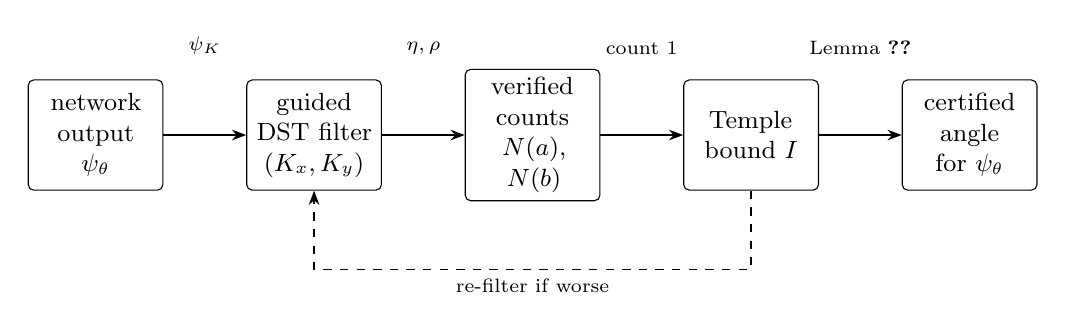
\begin{tikzpicture}[font=\small,
  box/.style={draw, rounded corners=2pt, align=center, inner sep=3pt,
              minimum height=14mm, text width=1.5cm, fill=white},
  arr/.style={-{Stealth[length=1.8mm]}, semithick},
  lab/.style={midway, above=0.9cm, font=\scriptsize}]
\node[box] (net)  {network output\\ $\psi_\theta$};
\node[box, right=1.05cm of net] (fil)
      {guided DST filter\\ $(K_x,K_y)$};
\node[box, right=1.05cm of fil] (cnt)
      {verified counts\\ $N(a)$, $N(b)$};
\node[box, right=1.05cm of cnt] (enc)
      {Temple\\ bound $I$};
\node[box, right=1.05cm of enc] (trn)
      {certified angle\\ for $\psi_\theta$};
\draw[arr] (net) -- (fil) node[lab] {$\psi_K$};
\draw[arr] (fil) -- (cnt) node[lab] {$\eta,\rho$};
\draw[arr] (cnt) -- (enc) node[lab] {count $1$};
\draw[arr] (enc) -- (trn) node[lab] {Lemma~\ref{lem:transport}};
\draw[arr, dashed] (enc.south) -- ++(0,-1.0) -| (fil.south)
      node[pos=0.25, below, font=\scriptsize] {re-filter if worse};
\end{tikzpicture}
\caption{The certification pipeline. The counters are called for each
candidate truncation pair; the filter keeps the narrowest enclosure among
those whose verified state index agrees with that of the unfiltered output
(Section~\ref{sec:filter}). The parenthesised arrows are the feedback that
makes the filter guided rather than fixed.}
\label{fig:pipeline}
\end{figure}

\subsection{A residual whose energy cannot leak}
\label{sec:leakage}

The training objective is the squared residual of \eqref{eq:residual}, a term
that fixes the scale, a boundary term and an energy term,
\begin{equation}
  \begin{split}
  \mathcal L(\theta) &=
  \operatorname*{mean}_{i}\big(\Hh\psi_\theta-\eta(\psi_\theta)\psi_\theta\big)_i^2
  + w_n\big(\langle\psi_\theta,\psi_\theta\rangle_h-1\big)^2 \\
  &\quad + w_b\big(\psi_\theta(a)^2+\psi_\theta(b)^2\big)
  + w_e\,\eta(\psi_\theta),
  \end{split}
  \label{eq:loss}
\end{equation}
with $(w_n,w_b,w_e)=(100,100,10)$ in one dimension. In two dimensions the
residual and the energy are evaluated on the unit iterate
$u=\psi_\theta/\norm{\psi_\theta}_h$, the Dirichlet condition is imposed
exactly by replacing the network output with
$\psi_\theta\leftarrow M\odot\psi_\theta$, where
$M(x,y)=(x-a)(b-x)(y-a)(b-y)$, so the boundary term vanishes identically and
$w_e=10$ is kept. In both dimensions $\eta(\psi_\theta)$ is the Rayleigh
quotient of the iterate, treated as a constant in the backward pass (it is the
minimizer over $E$, so detaching it leaves the gradient correct).

Four properties of \eqref{eq:loss} matter for certification. First, because
the residual uses the same $\eta$ as the certificate, the training objective
and the certified quantity coincide; a network trained on a different energy
(a learnable scalar, or a reference value) is optimizing a different residual,
and the certificate then measures that other objective. Second, the scale must
be fixed by an explicit term: without one $\psi\equiv0$ is an exact stationary
point of the residual, the loss is quadratic in the amplitude, and the amplitude is
left wherever the initialization put it---in our unnormalized two-dimensional
run it stayed as small as $\norm{\psi}^2=6\times10^{-5}$ while the shape had
already converged. One dimension fixes the scale with the penalty
$(\norm{\psi}_h^2-1)^2$; two dimensions divide by the norm inside the loss
instead. Third, the boundary condition: in one dimension the soft penalty of
weight $100$ leaves endpoint values of order $10^{-4}$ and contributes a
negligible part of the residual, whereas in two dimensions the same penalty is
diluted by the $O(1/N)$ fraction of boundary nodes and leaves the residual at
$O(1)$ (\ref{app:impl} records both failures), which is why the mask is used
there. Fourth, the energy term $w_e\eta$ is variational: it pulls the iterate
toward the lowest Rayleigh quotient and selects the ground state within the
near-null space of the residual; because $\eta$ is computed from the iterate,
it carries no external value.

\subsection{Certificate-guided spectral filtering}
\label{sec:filter}

A trained network contains high-frequency components that contribute almost
nothing to the Rayleigh quotient---which is stationary to first order---but
dominate the residual, which is not. Filtering them out turns an
uncertifiable output into a certifiable one. Under Dirichlet conditions the
natural basis is the tensor product of sine functions,
\begin{equation}
  \psi(x_i,y_j)\approx\sum_{p=1}^{K_x}\sum_{q=1}^{K_y} c_{pq}
  \sin\frac{p\pi x_i}{L}\sin\frac{q\pi y_j}{L},
  \label{eq:dst}
\end{equation}
with coefficients obtained by a two-dimensional type-I discrete sine
transform (DST-I) \citep{boyd2001}, which is separable, orthogonal up to a
diagonal scaling, and self-inverse.

The truncation order is chosen without any reference solution. For each
candidate pair $(K_x,K_y)$ on a prescribed schedule we filter, certify, and
record $(\text{width}, \text{state index})$. The selected pair is the one with
the smallest certified width \emph{among those whose certified state index
equals that of the unfiltered input}. The state-consistency constraint is not
optional: without it the filter happily projects an excited state onto the
ground-state sine, producing a much narrower certificate for the wrong
function. On the runs below the filter changes $\psi$ by a relative $L^2$
amount between $4\times10^{-6}$ and $2\times10^{-3}$, and reduces the residual
norm by a factor between $1.2$ and $7\times10^{9}$---below threefold in half
of the eighteen runs of the main sweep.

\subsection{Transporting the bound to the raw output}
\label{sec:transport}

The certificate of Section~\ref{sec:filter} refers to $\psi_K$, not to the
network output $\psi$. The gap can be bounded by an elementary inequality, so
that the network output itself receives a certified angle.

\begin{lemma}[Transport]\label{lem:transport}
Let $u=\psi/\norm{\psi}_h$, $u_K=\psi_K/\norm{\psi_K}_h$, and let $\varphi$ be
a unit eigenfunction. Then
\begin{equation}
  \sin\angle(u,\varphi)\ \le\ 2\norm{u-u_K}_h+\sin\angle(u_K,\varphi).
  \label{eq:transport}
\end{equation}
\end{lemma}
\begin{proof}
Since $\sin\angle(u,\varphi)=\norm{u-(u\cdot\varphi)\varphi}_h$ and
$\abs{(u_K-u)\cdot\varphi}\le\norm{u-u_K}_h$,
\begin{align*}
\sin\angle(u,\varphi)
&\le \norm{u-u_K}_h+\norm{u_K-(u_K\!\cdot\!\varphi)\varphi}_h
   +\abs{(u_K-u)\cdot\varphi}\\
&\le 2\norm{u-u_K}_h+\sin\angle(u_K,\varphi). \qedhere
\end{align*}
\end{proof}

The first term is computed from the two saved functions; the second is
Theorem~\ref{thm:dk} applied to $\psi_K$. The implementation uses the
conservative factor $2$ of \eqref{eq:transport}; a factor $1$ also follows from
the Lipschitz property of $\sin$ on $[0,\pi/2]$. The inequality is what allows
the tables to report a bound for the network output even when the unfiltered
output is not certifiable, and it answers the question "what exactly is being
certified?" with a number rather than a caveat.

\subsection{What a row of the results table contains}
\label{sec:row}

For each run the protocol reports: the certified state index and whether it
matches the target; the energy $\eta$ and the distance to an independently
computed $\lambda_h$; the residual before and after filtering; the certified
width before and after filtering; the certified angle bound, the transported
bound for the raw output, and the true discrete angle (computed only for
validation, never used by the protocol); the relative $L^2$ change caused by
the filter; and whether the enclosure contains the reference. Reporting the
raw and filtered columns side by side is essential: the first is what the
network guarantees by itself, the second is what can be certified in its
neighbourhood. Reporting only the second would overstate the network;
reporting only the first would understate what the protocol can do.

The one case in which this row does not exist is the degenerate level: there
is no single state to describe, and the certificate of
Section~\ref{sec:cert} refuses. Its replacement---a record for the invariant
subspace, with the multiplicity measured by counting---is the subject of
Section~\ref{sec:subspace}, and it is the object that the experiments of
Section~\ref{sec:deg-results} report.

\section{Certified clusters: subspaces, not individual states}
\label{sec:subspace}

The certificate of Section~\ref{sec:cert} answers the question ``which
eigenvalue is this state?''. At a degenerate level that question has no
answer: the problem does not define a single eigenvector, and a network that
solves it exactly returns an arbitrary element of a two-dimensional space
that depends on its seed. The honest object to certify is therefore the
\emph{invariant subspace}, and the honest statement is about the cluster of
eigenvalues it spans. This section gives that statement; it is what turns the
refusal of Section~\ref{sec:degeneracy} into a positive result.

Guaranteed two-sided bounds for eigenvalue clusters, multiplicity included,
already exist for conforming discretizations \citep{cances2020}. The setting
here differs in one respect that changes what has to be computed: a network
output is not a Galerkin projection, so no discretization parameter controls
its error and no saturation hypothesis relates it to an enriched space. Both
the cluster interval and the multiplicity must therefore be obtained from the
count, and the vector-side statement is a principal-angle bound that assumes
nothing about how the trial subspace was produced.

\subsection{The trial subspace and its residual}
\label{sec:sub}

Let $\psi_1,\dots,\psi_m\in\R^{|I|}$ be $m$ approximations---$m$ network
outputs, $m$ snapshots of one training run, or $m$ vectors from any other
source---and let $X=[x_1,\dots,x_m]$ be an orthonormal basis of their span,
$\langle x_i,x_j\rangle_h=\delta_{ij}$, obtained by symmetric
orthogonalization $X=\Psi G^{-1/2}$, $G_{ij}=\langle\psi_i,\psi_j\rangle_h$.
This choice matters: $G^{-1/2}$ is invariant under rotations of the input
basis, so the certificate depends on $\operatorname{span}\{\psi_j\}$ and not
on how the columns were ordered or mixed. If $G$ is singular the $m$ vectors
do not span an $m$-dimensional space and the certificate refuses before
computing anything else.

The compression of $\Hh$ to the trial subspace and its residual are
\begin{equation}
  M = X^{\mathsf T}\!\Hh X\in\R^{m\times m},\qquad
  R = \Hh X - X M ,
  \qquad \rho_F=\norm{R}_F ,
  \label{eq:rr}
\end{equation}
and the Rayleigh--Ritz pairs $(\theta_i,y_i)$, $My_i=\theta_iy_i$ with
$\theta_1\le\cdots\le\theta_m$, give the Ritz vectors $x_i\leftarrow X y_i$
(we reuse the symbol, since $\{Xy_i\}$ is again an orthonormal basis of the
same subspace) and the residual
\begin{equation}
  r_i=\Hh x_i-\theta_i x_i = R y_i ,\qquad
  \rho_i=\norm{r_i}_h,\qquad \sum_i \rho_i^2=\rho_F^2 .
  \label{eq:ritzres}
\end{equation}
Everything in \eqref{eq:rr}--\eqref{eq:ritzres} is computed from the
approximations alone.

\subsection{Two propositions}
\label{sec:props}

Write $N(\sigma)=\#\{i:\lambda_i<\sigma\}$ for the verified count of
Section~\ref{sec:counting}, and suppose an interval $(a,b)$ has been
\emph{verified} to contain exactly $m$ eigenvalues,
\begin{equation}
  N(b)-N(a)=m ,
  \label{eq:cluster}
\end{equation}
counting multiplicity. Let $V\subset\R^{|I|}$ be the corresponding invariant
subspace, $\dim V=m$, and let $P_V$ be the orthogonal projector onto it in
$\langle\cdot,\cdot\rangle_h$. Define the cluster margin
\begin{equation}
  \delta_i=\min(\theta_i-a,\,b-\theta_i),\qquad \delta=\min_i\delta_i .
  \label{eq:margin}
\end{equation}

\begin{lemma}[Cluster localization]\label{lem:cluster}
  Assume \eqref{eq:cluster}, $\theta_i\in(a,b)$ for all $i$, and
  $\rho_i<\delta_i$. Then
  \[
    \operatorname{dist}\big(\theta_i,\ \spec(\Hh)\cap(a,b)\big)\le\rho_i
    \qquad\text{for every }i .
  \]
\end{lemma}
\begin{proof}
  The pair $(x_i,\theta_i)$ is an approximate eigenpair in the sense of
  Definition~\ref{def:pair} with $\norm{x_i}_h=1$ and residual $r_i$, so
  Lemma~\ref{lem:weinstein} gives
  $\operatorname{dist}(\theta_i,\spec(\Hh))\le\rho_i$. Every eigenvalue of
  $\Hh$ outside $(a,b)$ is at distance at least $\delta_i$ from $\theta_i$,
  and $\rho_i<\delta_i$; hence the eigenvalue realizing the distance lies
  inside $(a,b)$.
\end{proof}

Lemma~\ref{lem:cluster} is the statement the single-state certificate cannot
make: it is valid no matter how close the $\theta_i$ are to each other,
because it never asks the interval to separate them. What it does not give is
an identification: when $\rho_i\ge\delta_i/2$ the intervals
$[\theta_i-\rho_i,\theta_i+\rho_i]$ may cover the same eigenvalue twice, and
the certificate makes no claim about which cluster eigenvalue belongs to
which Ritz value. At a degenerate level no such claim exists.

The angle between the trial subspace and $V$ obeys a Davis--Kahan inequality
in which the role of the spectral gap is played by the margin
\eqref{eq:margin}.

\begin{theorem}[Principal angle]\label{thm:angle}
  Under the hypotheses of Lemma~\ref{lem:cluster},
  \[
    \sin\Theta\big(\operatorname{span}X,\,V\big)\ \le\ \frac{\rho_F}{\delta},
  \]
  where $\Theta$ is the largest principal angle between the two subspaces.
\end{theorem}
\begin{proof}
  Let $\{\varphi_j\}$ be an orthonormal eigenbasis of $\Hh$ with
  $\Hh\varphi_j=\lambda_j\varphi_j$, and expand
  $x_i=\sum_j c_{ij}\varphi_j$. Since $\Hh x_i-\theta_i x_i
  =\sum_j(\lambda_j-\theta_i)c_{ij}\varphi_j$,
  \[
    \rho_i^2=\sum_j(\lambda_j-\theta_i)^2c_{ij}^2
    \ \ge\ \delta_i^2\!\!\sum_{j:\,\lambda_j\notin(a,b)}\!\! c_{ij}^2
    \ =\ \delta_i^2\,\big\lVert P_V^{\perp}x_i\big\rVert_h^2 ,
  \]
  because an eigenvalue outside $(a,b)$ differs from $\theta_i\in(a,b)$ by at
  least $\delta_i$. The Ritz vectors form an orthonormal basis of
  $\operatorname{span}X$, so
  \[
    \big\lVert P_V^{\perp}X\big\rVert_F^2
    =\sum_i\big\lVert P_V^{\perp}x_i\big\rVert_h^2
    \le\sum_i\frac{\rho_i^2}{\delta_i^2}
    \le\frac{\rho_F^2}{\delta^2},
  \]
  and the sine of the largest principal angle is the spectral norm of
  $P_V^{\perp}$ restricted to $\operatorname{span}X$, which is bounded by the
  Frobenius norm.
\end{proof}

Theorem~\ref{thm:angle} is the quantitative statement that a set of network
outputs spans the right subspace. For a single state ($m=1$) it reduces to
the Davis--Kahan bound \eqref{eq:dk} with $\delta$ in place of $\gamma$, which
is the same inequality shifted by $\eta$; the cluster version is not a
sharper theorem, it is the same theorem applied to the object that remains
well defined when the eigenvalue is degenerate.

\subsection{The cluster certificate}
\label{sec:cluster-alg}

The certificate is assembled exactly as in Section~\ref{sec:isolating}, with
$m$ in place of $1$:

\begin{enumerate}
\item \emph{Rank.} Form $G$ and refuse if it is numerically singular.
\item \emph{Rayleigh--Ritz.} Compute $M$, $\theta_i$, $\rho_i$, $\rho_F$
  from \eqref{eq:rr}--\eqref{eq:ritzres}.
\item \emph{Interval.} Propose $a$ and $b$ at the midpoints of the spectral
  gaps on either side of the block of $m$ approximate eigenvalues that
  matches $\{\theta_i\}$ (ARPACK is used to propose, never to decide), then
  \emph{verify} \eqref{eq:cluster}. If the proposal fails, bracket the two
  counting transitions by bisection and verify again; if that fails too, the
  refusal reason distinguishes a multiplicity mismatch from a subspace that
  spans more than one cluster.
\item \emph{Accept} if $\delta$ exceeds the resolution floor \eqref{eq:floor}
  and $\rho_i<\delta_i$ for every $i$; then report the interval $(a,b)$, the
  per-value enclosures $[\theta_i-\rho_i,\theta_i+\rho_i]$, and the angle
  bound of Theorem~\ref{thm:angle}. Otherwise refuse, with the reason.
\end{enumerate}

The cost is two verified counts---one sparse factorization each---one
$m\times m$ symmetric diagonalization, and $m$ applications of $\Hh$; it does
not grow with the number of requested eigenvalues beyond the $m$ matrix--vector
products, and it is negligible next to training.

Three properties are worth stating explicitly. First, $m$ is \emph{measured},
not asserted: the count decides whether the trial subspace has the dimension
the invariant subspace has, and a subspace that missed a state is refused
rather than certified with a smaller dimension. Second, Lemma~\ref{lem:cluster}
brackets each of the $m$ eigenvalues to within $\rho_i$ of a Ritz value, and the
multiplicity itself is verified only down to the counting resolution
\eqref{eq:floor}; both hold independently of how accurate the network is: a
poor subspace yields a poor angle bound but never a wrong multiplicity. Third, the interval may
contain a block of adjacent distinct eigenvalues; degeneracy is the case that
motivates the construction, not a special case of it.

The refusal reasons are meant to be actionable, and that suggests a
procedural use of the certificate. A multiplicity mismatch says that the trial
subspace missed a state of the cluster or covered more than one cluster, and
tells the user how many vectors to supply or how to split them;
$\rho_i\ge\delta_i$ says that the subspace is not an accurate enough
approximation and that more training is required; a span whose second
direction is the difference of nearly identical outputs says that the runs
collapsed and that a further direction must be forced, which is done by
deflating the accepted outputs as well and retraining. The loop
\emph{train, certify, deflate, retrain} is what produced the accepted neural
pair of Section~\ref{sec:deg-results}, and its termination argument is the one
familiar from deflated eigensolvers: each accepted direction is projected out
of the residual that the next run minimises.

\begin{remark}[What a cluster certificate does not say]
\label{rem:cluster-not}
It does not say that $\theta_i$ approximates $\lambda_i$ in the matching
order, and it does not give an $O(\rho^2)$ enclosure: for $m=1$ the
Kato--Temple bound of Theorem~\ref{thm:temple} is sharper and should be
preferred whenever its hypothesis holds. It also does not resolve eigenvalues
that the counting cannot separate, exactly as in \eqref{eq:floor}; what it
does is to make the resolution floor the \emph{only} obstacle, removing the
structural one.
\end{remark}

\begin{remark}[Do independent runs span a degenerate level?]\label{rem:two}
It is tempting to certify a degenerate level by training $m$ networks and
certifying their span, and the answer depends on the data rather than on the
construction. In our experiments three of four independent runs collapsed onto
the same symmetry-broken representative (pairwise overlap $>0.9999$) while the
fourth found the orthogonal partner. The certificate accepted every pair
containing the fourth run, with bounds of $5.6$--$6.3\times10^{-3}$; it refused
the two remaining pairs of near-identical outputs, $(0,1)$ and $(1,2)$, whose
second directions are differences of norm $2.4\times10^{-3}$ and
$6.7\times10^{-3}$---for both, the Ritz residual of that direction ($16.3$ and
$7.5$) exceeds the margin ($6.1$ and $7.2$), so the span contains no invariant
subspace of dimension two; and it accepted the pair $(0,2)$, which omits the
fourth run, only with a bound two orders of magnitude looser ($0.68$), which
is the honest signal that its second direction was mostly noise. The certified
object is the subspace, not the individual vector, and the certificate sorts
sets of outputs by how much of a second direction they actually contain. When the answer is negative the
second direction can be forced by deflating the first output as well, as in
Section~\ref{sec:deg-results}.
\end{remark}

\section{Implementation}
\label{sec:software}

\subsection{Structure}

The package is organised in three layers. The \texttt{physics} layer
(pure NumPy) provides analytic references and a Numerov integrator used to
cross-check them. The \texttt{solver} layer contains the samplers, networks,
losses and trainer, and---separately from training---the certification
modules \texttt{certify} (1D), \texttt{filtering} (1D DST filter),
\texttt{certify2d} (2D inertia counting and certificates),
\texttt{filtering2d} (2D DST filter and transport) and
\texttt{certify\_subspace} (cluster and invariant-subspace certificates,
Section~\ref{sec:subspace}), \texttt{certified\_count} (directed-rounding
counting and the certified eigenvalue brackets of
Section~\ref{sec:certified}) and \texttt{continuous\_bound} (the variational
bound of Section~\ref{sec:variational}). The \texttt{scripts}
directory contains one driver per experiment plus the aggregation and
reporting utilities; every table in this paper is generated by a script from
saved JSON, not transcribed by hand.

The certification modules do not import PyTorch and do not require a trained
network: they operate on an array of samples and the grid. This is deliberate,
because the certificate must remain meaningful if the training stack changes.

\subsection{Application programming interface}

Table~\ref{tab:api} lists the entry points a user needs; everything else is
built from them. The three certificate calls and the three counting calls are
the whole interface to the numerics.

\begin{table}[t]
\centering
\footnotesize
\setlength{\tabcolsep}{2pt}
\begin{tabular}{@{}ll@{}}
\toprule
Call & Purpose \\
\midrule
\texttt{certify\_eigenpair(psi, x, V, isolate=True)} & 1D certificate \\
\texttt{count\_eigenvalues\_below(x, V, sigma)} & 1D Sturm count \\
\texttt{guided\_filter(psi, x, V)} & 1D filter + re-certification \\
\texttt{certify\_eigenpair\_2d(psi, grid, isolate=True)} & 2D certificate \\
\texttt{count\_eigenvalues\_below\_2d(grid, sigma)} & 2D Sylvester count \\
\texttt{guided\_filter\_2d(psi, grid)} & 2D filter + re-certification \\
\texttt{transported\_angle\_bound\_2d(\dots)} & Lemma~\ref{lem:transport} \\
\texttt{certify\_subspace\_1d(psis, x, V)} & 1D cluster certificate \\
\texttt{certify\_subspace\_2d(psis, grid)} & 2D cluster certificate \\
\texttt{certified\_sturm\_count\_1d(x, V, sigma)} & count, directed rounding \\
\texttt{certified\_separable\_count\_2d(grid, sigma)} & separable 2D count \\
\texttt{certified\_eigenvalue\_brackets\_1d(...)} & certified eigenvalue brackets \\
\texttt{p1\_rayleigh\_bound(x, V, psi)} & upper bound on $\lambda_1(\mathcal H)$ \\
\texttt{q1\_rayleigh\_bound\_2d(x, y, V, psi)} & the same in two dimensions \\
\texttt{principal\_angle(X, exact, h)} & validation only, not a certificate \\
\bottomrule
\end{tabular}
\caption{Main entry points. A certificate is returned as a record with the
energy, the enclosure, the verified gap, the state index, the angle bound and,
when certification is refused, the reason.}
\label{tab:api}
\end{table}

Every certificate is a plain record (a frozen dataclass), so it serialises to
JSON without custom code; the experiment drivers store one record per run. A
refused certificate carries a machine-readable reason---``no isolating
interval exists'', ``gap below resolution floor'', ``Temple condition fails'',
``energy outside the interval''---which is what makes the refusal auditable
rather than a silent \texttt{None}.

A self-contained example, \texttt{examples/certify\_demo.py}, exercises both
paths in about four seconds and without PyTorch: it certifies the analytic trial
function $\mathrm{e}^{-x^2/2}$ of the harmonic oscillator, then reproduces the
refusal-then-subspace sequence of Section~\ref{sec:deg-results} on a
$61\times61$ box, where one member of the degenerate pair is refused as a
state and the pair is certified as a cluster.

\subsection{Drivers and reproducibility}

The experiments of Section~\ref{sec:results} are produced by the commands
below.

\noindent\begin{minipage}{\linewidth}
\footnotesize
\begin{verbatim}
python scripts/run_seed_sweep.py --jobs 6 --threads 4   # 1D, seeds 0-2
python scripts/run_seed_sweep_2d.py --jobs 2            # 2D, seeds 0-2
python scripts/filter_certificates.py                   # 1D certify
python scripts/filter_certificates2d.py                 # 2D certify
python scripts/exp7_degeneracy_2d.py                    # degeneracy
python scripts/exp8_subspace_certificate.py             # clusters
python scripts/exp9_resolution_boundary.py              # floor
python scripts/discretization_study_2d.py --sizes 41 61 81 101 121
python scripts/go_nogo.py ; python scripts/leakage_audit.py
python scripts/multistate_report.py
python scripts/bench_count.py                           # timings
python scripts/dense_reference_2d.py                    # 2D reference
python scripts/appendix_failures.py --variant soft_boundary
python scripts/residual_vs_error.py runs/appendix_failures/unnormalized
python scripts/lapack_reference_widths.py
python scripts/directed_count_report.py
python scripts/continuous_bound.py
python scripts/continuous_bound.py --alignment   # finite well, O(h) sign
python paper/make_tables.py ; python paper/make_figures.py
\end{verbatim}
\end{minipage}

\vspace{0.3em}\noindent Each driver writes a JSON manifest with the wall-clock time of every job, so
the runs are reproducible and the cost figures below are measured rather than
estimated. The 1D runs (10\,000 epochs, grid of 2001 points, network
$64\times3$) take $30$--$45$\,s each on a laptop CPU; the 2D runs
($6000$ epochs, $81\times81$ grid, network $64\times4$) take $99$--$109$\,s
each, manifest times that include start-up and saving.
Certification itself is negligible in both cases. One count
takes $0.4$\,ms at $N=2001$ and $0.034$\,s at $81\times81$ (median of twelve
timed calls, \texttt{scripts/bench\_count.py}); a full certificate---interval
proposal, verified count, and Temple bound---takes $0.074$\,s at $N=2001$,
which is some two hundred counts, and $0.19$\,s at $81\times81$, which is six,
and a complete certificate-guided scan costs $2.6$\,s over the $27$
one-dimensional cutoff orders; in two dimensions the timed benchmark records
$16$\,s for an $81$-candidate scan, and the $30$- and $62$-candidate scans of
the experiments, which examine fewer candidates, scale from it to about $6$
and $12$\,s. The count inherits
the scaling of the sparse factorization it reads: $3$\,ms at $41\times41$,
$0.03$\,s at $81\times81$ and $0.85$\,s at $201\times201$, still small
against a training run on the same grid.

\subsection{Numerical safeguards and tests}

The safeguards described in Section~\ref{sec:counting} are assertions in the
code, not comments: a count that fails the identity-permutation or pivot test
is retried with a perturbed shift and then reported as unavailable. The test
suite (143 tests, run with or without \texttt{pytest}) locks the following
properties, among others:
\begin{itemize}
\item the 1D Sturm count and the 2D Sylvester count agree element by element
  with dense eigen-decomposition on small grids;
\item an exact discrete eigenvector receives a valid certificate whose
  enclosure contains the reference eigenvalue and whose width is at the
  round-off floor;
\item a degenerate eigenvector is refused (Section~\ref{sec:deg-results}),
  while the pair of exact eigenvectors spanning the level is certified as a
  cluster;
\item a rank-deficient set of trial vectors, a single member of a degenerate
  pair, and a cluster whose multiplicity disagrees with the verified count are
  all refused, and a rotated basis of the same subspace returns the same
  certificate;
\item the DST-I used by the filter is its own inverse;
\item the guided filter recovers the exact sine mode of a box potential from a
  perturbed input;
\item the transported bound of Lemma~\ref{lem:transport} dominates the true
  angle;
\item the directed-rounding count agrees with dense eigen-decomposition on
  every shift where it does not refuse, is monotone in the shift, and
  \emph{refuses} at a shift equal to an eigenvalue and for a non-separable
  two-dimensional potential;
\item the variational bound exceeds the true continuous energy for the box
  and the harmonic oscillator, its error contracts at the observed $O(h^2)$
  rate, its quadrature check rejects a kink it was not told about---and, in
  two dimensions, a non-polynomial potential---while accepting the quartic
  anharmonic one, and the two-dimensional Q1 bound equals the sum of the two
  one-dimensional bounds on a non-square grid.
\end{itemize}
The third item deserves emphasis: a test that only asserted ``the certificate
is valid'' would have passed on a version of the code that produced a
spuriously narrow interval for a degenerate state. The test asserts the
refusal.

\section{Certified counting and the continuous operator}
\label{sec:certified}

Sections~\ref{sec:cert}--\ref{sec:subspace} certify quantities computed from
$\Hh$ in double precision, and Section~\ref{sec:fp} names two limitations: the
count $N(\sigma)$ is a combinatorial object read off a floating-point
factorization, and every statement refers to $\Hh$ rather than to
$\mathcal H$. This section attacks both with two constructions that turn out
to be cheap: a directed-rounding count, which removes the first limitation in
one dimension and in two whenever the potential is separable, and a
variational bound on the continuous eigenvalue, which removes half of the
second---the upper side---for every potential and needs no reference solution
and no interpolation constant.

\subsection{Directed rounding}

An interval $[a,b]$ represents every real in it; an operation returns
$\{x\circ y : x\in[a,b],\,y\in[c,d]\}$ rounded outward. The implementation is
a few dozen lines: each endpoint is moved one ulp outward with
\texttt{nextafter}, which is enough because IEEE\,754 arithmetic is correctly
rounded, so the exact result of a single operation lies within half an ulp of
the computed one. This is not higher-precision arithmetic---the precision is
still double---but every rounding is forced to the side that preserves the
statement.

What the resulting count certifies must be stated carefully, because it is
easy to overclaim. The certified matrix is the one the implementation actually
stores: diagonal entries $h^{-2}+V_i$, off-diagonals $-\tfrac12h^{-2}$, each
taken as an exact real number. A certified count is therefore a theorem about
\emph{that} symmetric tridiagonal matrix. Any difference between it and the
matrix a reader would write down from \eqref{eq:Hh} is a modelling question
(rounding of $h^{-2}$, of the potential samples), not a counting question.

\subsection{One dimension: pivots rather than determinants}

For a symmetric tridiagonal $T=\Hh-\sigma I$ with diagonal $a_k$ and
off-diagonal $b_k$, the number of eigenvalues below $\sigma$ is the number of
negative pivots in the $LDL^\top$ factorization, i.e.\ of the recurrence
\begin{equation}
  q_1 = a_1-\sigma,\qquad q_k = (a_k-\sigma) - \frac{b_{k-1}^2}{q_{k-1}} ,
  \label{eq:pivot}
\end{equation}
by Sylvester's law of inertia. The determinant recurrence
$d_k=(a_k-\sigma)d_{k-1}-b_{k-1}^2d_{k-2}$ computes the same sign pattern in
exact arithmetic, and we tried it first: it is unusable. In intervals the
relative width of $d_k$ exceeds $1$---so the interval contains zero and the
sign is undecidable---after $35$ to $45$ steps, on every one of the $363$
scan shifts at $N=2001$ (\texttt{runs/directed\_count/stats.json}). The
determinant cancels catastrophically because it alternates in sign and nearly
does so at the scale of the spectrum's bulk. Equation~\eqref{eq:pivot} avoids
this: when the pivot is resolved, the quotient $b^2/q_{k-1}$ is a small
correction to $a_k-\sigma$, and the interval stays narrow to the end of the
recurrence. The cost is one division per node, which must be refused when the
pivot interval straddles zero.

That refusal is the whole point. A count that cannot be decided is reported as
uncertified with the index of the offending pivot, and the caller must handle
it; it is never rounded to an integer. On three potentials at $N=2001$, over
$121$ shifts spanning the low spectrum, $361$ of $363$ shifts were certified
and every certified value equals both the floating-point count and the dense
eigen-decomposition (\texttt{runs/directed\_count/stats.json}). Both refusals
are at the scan's last shift, which in each scan coincides exactly with an
eigenvalue in double precision---precisely the case a rigorous implementation
must refuse---and the refusal names the offending pivot (index $999$). A
median count costs $5$\,ms, against
$0.4$\,ms for the floating-point version (\texttt{runs/\_bench/count\_timing.json})---a
factor of thirteen.

Two further uses follow. Bisecting on the certified count produces a
\emph{certified bracket} for a discrete eigenvalue; when the bisection
reaches the resolution of the recurrence it stops and returns the last
verified bracket instead of failing. This is what the driver
\texttt{scripts/continuous\_bound.py} reports in the $\lambda_h$ column of
Table~\ref{tab:continuous} for the one-dimensional rows and, through the
Kronecker route described below, for the two separable two-dimensional
potentials as well; only the anharmonic potential's
$\lambda_h$ is a sparse-factorization eigenvalue rather than a certified
bracket.

\subsection{Two dimensions: a Kronecker sum, and why not elimination}

The obvious two-dimensional analogue is a banded $LDL^\top$ in intervals. It
does not work, and the failure is quantitative rather than a matter of
implementation: the elimination divides by pivots and the interval width is
amplified at each step, so pivots straddle zero long before the factorization
ends. At $361$ unknowns, $6$ of $10$ shifts could not be counted; the relative
pivot width reached $0.93$ immediately before one of the refusals, and the
earliest refusal came at step $174$ of the elimination, where the width was
$0.44$ (\texttt{runs/directed\_count/stats.json}). Symmetric pivoting does
not repair this, because the difficulty is overestimation, not a zero pivot.

For a separable potential, however, no elimination is needed at all. If
$V(x,y)=V_x(x)+V_y(y)$ then
\begin{equation}
  \Hh = A_x\otimes I + I\otimes A_y
  \label{eq:kron}
\end{equation}
exactly, with $A_x,A_y$ the one-dimensional operators on the two grids, so
$\spec(\Hh)=\{\mu_i+\nu_j\}$ and
\begin{equation}
  N(\sigma) = \#\{(i,j): \mu_i+\nu_j < \sigma\}.
\end{equation}
Each one-dimensional eigenvalue is bracketed by the certified count of the
previous subsection, and the two-dimensional count is a comparison of sums. A pair whose sum interval straddles $\sigma$ makes the count refuse. That
is not a property of degenerate levels as such---any $\sigma$ inside the
certified bracket of a pair refuses---but in the cluster protocol the scan
places $\sigma$ on a level, and for the box, whose spectrum has
multiplicities, the midpoint of a degenerate pair is the eigenvalue
itself. On the harmonic and box potentials at $81\times81$, all
$25$ shifts of a scan were certified with zero disagreements against the
floating-point inertia count, at $18$\,ms per count. The non-separable
anharmonic potential is refused outright, with a reason, rather than
silently falling back to floating point. Bisecting on this count yields
certified brackets for the two-dimensional eigenvalues themselves---widths
of $1.4$--$6.0\times10^{-11}$ for the harmonic oscillator and
$3.7\times10^{-10}$--$2.5\times10^{-9}$ for the box between $41$ and $101$
points per side---which is where the two-dimensional $\lambda_h$ of
Table~\ref{tab:continuous} comes from.

\subsection{A variational bound for the continuous operator}
\label{sec:variational}

Every statement so far concerns $\Hh$. The gap to $\mathcal H$ was left as an
open item because the standard routes---an eigenvalue-perturbation estimate
with an explicit $O(h^2)$ constant, or a homotopy/Newton enclosure of the
elliptic problem---need regularity or pointwise bounds that a trained network
does not supply.

One direction needs none of that. By the min--max principle,
\begin{equation}
  \lambda_1(\mathcal H) = \min_{u\in H^1_0}\ \frac{\tfrac12\int u'^2 + \int V u^2}{\int u^2}
  \;\le\; R(u)
  \qquad\text{for every } u\in H^1_0 ,
  \label{eq:minmax}
\end{equation}
so \emph{any} conforming trial function yields an upper bound on the
continuous ground-state energy. The P1 (bilinear, in 2D) interpolant of a
sampled function is continuous and vanishes at the boundary, hence is in
$H^1_0$: the network's own eigenfunction, once interpolated, is a legitimate
trial function. No reference solution, no grid operator and no interpolation
constant enters. This is the precise sense in which the certificate now
reaches the continuous operator.

The arithmetic of \eqref{eq:minmax} must be distinguished from its
mathematics. In exact arithmetic the stiffness term is exact on our grids:
piecewise constant in one dimension, and a polynomial of degree two in each
variable in two dimensions, which the Gauss rule integrates exactly. The
potential term is integrated by Gauss quadrature on each element, which is
exact when $V u^2$ is a polynomial of low degree there---true for the
harmonic oscillator, the box, and, with the breakpoints supplied as element
boundaries, the finite well. Rather than trust the hypothesis, the code
evaluates the potential integral under two Gauss rules of different order and
refuses the bound whenever the two intervals fail to intersect; a kinked
potential whose kink lies inside an element is caught by that check. What the
code does \emph{not} do is evaluate the element integrals in interval
arithmetic: the accumulations are outward-rounded, with a padding that grows
with the number of terms, but the element-level arithmetic and the evaluation
of $V$ at the Gauss nodes are ordinary double precision. For the potentials
here that rounding is a few ulp, orders of magnitude below the padding the
summation already carries and eleven orders below the bracket it is compared
with; it is nevertheless a gap, and a user who needs it closed must supply an
interval evaluation of $V$. The one-sided statement---$\lambda_1(\mathcal H)
\le R(\psi_h)$---is then a theorem about the computed quotient up to that
rounding, and exactly a theorem about the quotient in exact arithmetic.

Table~\ref{tab:continuous} applies \eqref{eq:minmax} to the coarse and fine
ends of each of the six problems. Two columns matter. The bracket
$R(\psi_h)-\lambda_h$ contracts by the ratio that $O(h^2)$ predicts when the
grid is refined: $6.2$--$6.3$ for the three two-dimensional potentials between
$41$ and $101$ points per side (prediction $6.25$) and $56$--$64$ for the
harmonic oscillator and the infinite well between $501$ and $4001$ (prediction $64$;
the finite well has no such ratio, because its bracket changes sign, as
discussed below). At the
coarse grid the reference value lies between the two columns in all five
cases where it is known; at the fine grid in four of five, the exception
being the finite well, discussed below. For the
two-dimensional anharmonic potential, where no reference exists, the bracket
is a \emph{one-sided} statement: the true ground-state energy is at most the
tabulated $R(\psi_h)$.

\begin{table}[t]
\centering
\footnotesize
\setlength{\tabcolsep}{2pt}
\begin{tabular}{@{}llrrll@{}}
\toprule
Potential & $N$ & $\lambda_h$ & $R(\psi_h)$ & $\lambda^\star$ & in \\
\midrule
Harmonic & 501 & 0.4999819994 & 0.5000180013 & 0.5000000083 & \checkmark \\
Harmonic & 4001 & 0.4999997318 & 0.5000002813 & 0.5000000083 & \checkmark \\
Infinite well & 501 & 4.9347859593 & 4.9348184354 & 4.9348022005 & \checkmark \\
Infinite well & 4001 & 4.9348016381 & 4.9348024542 & 4.9348022005 & \checkmark \\
Finite well & 501 & -48.9981281228 & -48.9787820344 & -48.9810479595 & \checkmark \\
Finite well & 4001 & -48.9773754207 & -48.9809713144 & -48.9810479595 & $\times$ \\
\midrule
Harmonic (2D) & 41 & 0.9993927428 & 1.0021728615 & 1.0007820274 & \checkmark \\
Harmonic (2D) & 101 & 1.0005601465 & 1.0010042177 & 1.0007820274 & \checkmark \\
Box (2D) & 41 & 9.8645320539 & 9.8746788339 & 9.8696044011 & \checkmark \\
Box (2D) & 101 & 9.8687926854 & 9.8704161708 & 9.8696044011 & \checkmark \\
Anharmonic (2D) & 41 & 1.0962601793 & 1.1002100307 & -- & -- \\
Anharmonic (2D) & 101 & 1.0979179490 & 1.0985487577 & -- & -- \\
\bottomrule
\end{tabular}

\caption{Discrete eigenvalue $\lambda_h$ (the midpoint of a directed-rounding
bracket wherever the potential is separable---all one-dimensional rows, and
the harmonic and box in two dimensions; a sparse-factorization eigenvalue
for the anharmonic potential) and the
variational upper bound $R(\psi_h)$ of \eqref{eq:minmax} on the P1/Q1
interpolant of the discrete eigenvector. The final column asks whether the
reference value $\lambda^\star$ lies in $[\lambda_h,R(\psi_h)]$; ``--'' means
no reference is known. The finite well's failure at $N=4001$ is real---it
fails already at $N=2001$---and is discussed in the text.}
\label{tab:continuous}
\end{table}

\subsection{The two sides are not symmetric}

The upper bound is unconditional; the lower side is not, and one of our own
potentials shows why. The finite well has a discontinuous $V$, so the local
truncation error of the three-point stencil is $O(h)$---not $O(h^2)$---near the
jump, and its \emph{sign depends on where the jump falls relative to the
grid}. Across the twelve grids $N=1000,\dots,1011$ on the same well, the
discrete ground energy lies above the continuous value on six and below on
six, with errors up to $1.4\times10^{-2}$ and no monotone decay
(\texttt{runs/continuous\_bound/alignment.json}). Figure~\ref{fig:alignment}
shows the twelve signs.

\begin{figure}[t]
\centering
\begin{tikzpicture}
\begin{axis}[
  width=0.78\linewidth, height=0.40\linewidth,
  xlabel={grid points $N$}, ylabel={$\lambda_h-\lambda^\star$},
  ymin=-0.017, ymax=0.017,
  xtick={1000,1002,1004,1006,1008,1010},
  tick label style={font=\footnotesize},
  label style={font=\small},
  grid=major, grid style={dotted,gray!45},
  axis line style={gray!70},
]
\addplot+[ycomb, mark=*, mark size=1.1pt, thick, blue!55!black]
  table[col sep=comma, x=N, y=error]
  {figures/data/finite_well_alignment.csv};
\draw[black!55, dashed, line width=0.4pt]
  (axis cs:999.5,0) -- (axis cs:1011.5,0);
\end{axis}
\end{tikzpicture}
\caption{The finite well on twelve consecutive grids: the same potential,
only the grid moved. The discrete ground energy alternates above and below
the continuous value, with no trend in $N$, so the sign of the
discretization error is a property of the alignment of the jump with the
grid rather than of the grid size. Plotted from
\texttt{runs/continuous\_bound/alignment.json}; the $N=4001$ point discussed
in the text lies outside the window.}
\label{fig:alignment}
\end{figure}

The mechanism is visible on a single grid. At $N=4001$ the jump falls exactly
on a node, and the value that node receives---inside the well or outside---is
the whole error: keeping the grid and sampling that one point as $-50$ instead
of $0$ moves $\lambda_h$ by $7.4\times10^{-3}$, from $+3.67\times10^{-3}$ to
$-3.73\times10^{-3}$, straddling the true value. The convention used in the
table (the node outside, so the well is one grid point narrower) is what puts
$\lambda_h$ above $\lambda^\star$, and is why the finite-well bracket of
Table~\ref{tab:continuous} does not contain it at the finer grid. Neither
convention is more accurate; the discrete energy of a discontinuous potential
at an aligned grid is not a variationally consistent estimate of the
continuous one, and no amount of rounding control changes that.

The lesson is not that the count is wrong---it is certified, and it is a
certified statement about the stored matrix---but that a certified discrete
calculation does not by itself certify a continuous quantity when the method
is not variationally consistent. The same grid on a smooth potential behaves:
for the harmonic oscillator the discrete value is below the continuous one at
every grid we tried.

For the infinite well the lower side can also be made rigorous, and by an elementary
inequality rather than a numerical observation. On $[0,1]$ with $h=1/(n+1)$,
the eigenvalues of $\Hh=-\tfrac12\Delta_h$ are
\begin{equation}
  \lambda_j^{(h)} = \frac{2}{h^2}\sin^2\frac{j\pi h}{2},
  \qquad
  \lambda_j = \frac{j^2\pi^2}{2},
  \label{eq:sine}
\end{equation}
and $\sin\theta\le\theta$ gives $\lambda_j^{(h)}\le\lambda_j$ for every $j$ and
every $h$. In two dimensions the same argument applies along each axis, and
since the ordering of sums is preserved, $\lambda^{(h)}_j\le\lambda_j$ holds
for the entire spectrum of the two-dimensional box. There both ends are
provable: the sine inequality puts the discrete eigenvalue below
$\lambda^\star$, \eqref{eq:minmax} puts $\lambda^\star$ below $R(\psi_h)$, and
the certified bracket locates the discrete eigenvalue to
$2.5\times10^{-9}$---five orders of magnitude inside the margin
$8\times10^{-4}$ between the two bounds at the finer grid, so the tabulated
midpoint can be replaced by the bracket's lower endpoint without changing the
conclusion. For the other potentials
we do not have a lower bound, and we do not claim one: the honest summary is
that \eqref{eq:minmax} makes the continuous eigenvalue certifiable from above
for every potential---for the harmonic oscillator the discrete value is below
the continuous one at every grid we tried (\texttt{bound.json})---and from
below only where a comparison principle is available.

\subsection{What this changes}

The protocol of Section~\ref{sec:protocol} is unchanged, and so is the cluster
construction: what limits a certificate at a degenerate level is the
resolution at which two shifts can be separated, and wherever the count is
certified, directed rounding replaces ``double precision with guards'' by
``provable or refused'' at that same resolution. The experiments of Section~\ref{sec:results} still count in
floating point with the guards of Section~\ref{sec:counting}, at $0.4$\,ms
rather than $5$\,ms per count: the two agree on every shift at which the
certified count does not refuse, and the certified function takes the same
arguments when the guarantee rather than the speed is wanted. What does change
is the answer to the question a referee
should ask of any certified eigenvalue of a \emph{discretized} problem: how
far is this from the equation you actually wanted to solve? The upper bound
answers it with a number, for every trial function the practitioner already
has---including the trained one---and it is the only one of the two sides that
holds without a comparison principle.

\section{Numerical experiments}
\label{sec:results}

\subsection{Setup}
\label{sec:setup}

\paragraph{Potentials} In one dimension we use the harmonic oscillator
$V=\tfrac12x^2$ on $[-6,6]$, the infinite square well on $[0,1]$, and a finite
square well of depth $V_0=50$ and half-width $1$ on $[-8,8]$. The first two
have closed-form spectra, which we use only to construct training references
and to label the runs; the certificate never sees them. In two dimensions we
use $V=\tfrac12(x^2+y^2)$ on $[-3,3]^2$, the box $[0,1]^2$, and the
non-separable potential $V=\tfrac12(x^2+y^2)+\tfrac12x^2y^2$ on $[-3,3]^2$,
for which no closed form is used at all: the certificate does not need one and
neither does the reference, which is the dense LAPACK solve described under
\emph{References} below.

\paragraph{Networks and training} One-dimensional runs use an MLP of width
64 and depth 3 with Fourier features, $10^4$ epochs of Adam, and a grid of
2001 points; two-dimensional runs use width 64, depth 4, no Fourier features,
6000 epochs and an $81\times81$ grid. The loss is \eqref{eq:loss}. Three seeds
(0, 1, 2) are run for every potential; all reported ranges are over seeds.

\paragraph{References} Every enclosure is compared against a value obtained
independently of both the network and the certificate: in 1D by LAPACK's
symmetric tridiagonal solver, evaluated as the Rayleigh quotient of the
returned vector (the raw LAPACK eigenvalue has absolute error of order
$\varepsilon\norm{\Hh}$, from $7\times10^{-12}$ on the finite-well grid to
$2\times10^{-9}$ on the box grid, at least as large as the narrowest widths
being tested); in
2D by a dense LAPACK decomposition of the full $6241\times6241$ matrix. ARPACK
is used in 2D only to propose interval endpoints; it agrees with the dense
reference to all ten printed digits and is never the reference itself. The
reference is used for validation only; it is never an input to the
certificate.

\subsection{One-dimensional ground states}
\label{sec:1d}

Table~\ref{tab:1d} summarises the nine ground-state runs with the
leakage-free (Rayleigh-quotient) residual.

\begin{table}[t]
\centering
\small
\setlength{\tabcolsep}{2pt}
\begin{tabular}{lccc}
\toprule
 & Harmonic & Infinite well & Finite well \\
\midrule
raw cert. & 2/3 & 2/3 & 3/3 \\
$|E_f-\lambda_h|$ & $1.6\times10^{-6}$--$7.4\times10^{-5}$ & $3.7\times10^{-14}$--$1.8\times10^{-13}$ & $(1.3\text{--}7.7)\times10^{-4}$ \\
width, raw & $0.143$--$0.65$ & $(5.9\text{--}6.2)\times10^{-4}$ & $0.553$--$2.76$ \\
width, filtered & $2.7\times10^{-5}$--$9.3\times10^{-4}$ & $9.9\times10^{-12}$ & $0.374$--$0.729$ \\
angle bound & $3.7\times10^{-3}$--$2.2\times10^{-2}$ & $(7.3\text{--}7.5)\times10^{-10}$ & $0.56$--$0.835$ \\
contains $\lambda_h$ & 3/3 & 3/3 & 3/3 \\
\bottomrule
\end{tabular}

\caption{One-dimensional ground states, three seeds per potential, 2001-point
grid, $10^4$ epochs. ``raw cert.'' is the number of seeds for which the
unfiltered network output is certifiable. Widths and angle bounds are from the
filtered certificate; ``contains'' counts the enclosures that contain the
independently computed $\lambda_h$.}
\label{tab:1d}
\end{table}

All nine enclosures contain $\lambda_h$, and after filtering all nine runs are
certifiable. The raw certification rate is $7/9$: two networks produce
outputs whose residual is too large relative to the spectral gap for the
Temple condition \eqref{eq:templecond} to hold, which is exactly the situation
in which an unfiltered claim would have to be withheld.

The three potentials separate sharply.
\begin{itemize}
\item \emph{Harmonic.} Certified widths $2.7\times10^{-5}$ to
  $9.3\times10^{-4}$, angle bounds $3.7\times10^{-3}$ to
  $2.2\times10^{-2}$~rad against true angles of $9\times10^{-4}$ to
  $5\times10^{-3}$~rad. The
  enclosure is between 5 and 19 times wider than the true error---usable, and
  the only potential where it is.
\item \emph{Infinite well.} Width $9.9\times10^{-12}$, i.e.\ at the
  round-off floor of the interval endpoints. This is not evidence that the
  network is accurate to $10^{-11}$; it is evidence that after filtering the
  network output is a single sine mode, and the residual of that mode is
  limited only by the arithmetic. We report it as a validation of the
  mechanism, not as a precision claim.
\item \emph{Finite well.} Widths $0.37$--$0.73$ and angle bounds up to
  $0.84$~rad, against a true energy error of $1.3$--$7.7\times10^{-4}$ and a
  true angle of $10^{-3}$--$3\times10^{-3}$~rad. The enclosure is correct and
  useless: the ratio of certified width to true error is $10^{3}$. The reason is structural---the kink at
  $|x|=1$ makes the discrete eigenvalue converge at first order, and the
  network's short-wavelength error near the interface is indistinguishable,
  from the inside, from a genuine high-wavenumber component of the exact
  eigenfunction. No amount of training removes the ambiguity; only a
  different discretization (or a bound that uses regularity) would.
\end{itemize}

This spread is the main practical message of the paper: a certificate is not
uniformly tight, and the ratio between certified width and true error is
itself a quantity that must be reported.

\subsection{What the filter does}
\label{sec:filter-results}

Figure~\ref{fig:filter}(a) shows the certified width as a function of the
truncation order $K$ for one run per potential. The harmonic curve has the
shape of a bias--variance trade-off: at $K=8$ the truncation discards
legitimate structure and the width is $0.31$; the width falls by four orders
of magnitude to $3.0\times10^{-5}$ at $K=15$, stays flat through $K=20$, and
then grows steadily as noise modes re-enter the residual, reaching $0.59$ at
$K=1500$. The minimum is selected without any reference, from the certificate
alone, and it coincides with the point beyond which the residual is dominated
by components that do not affect the energy. For the infinite well the
minimum is at $K=1$ and the curve is monotone increasing: the exact state is
the first sine mode and every additional mode is noise. For the finite well
the minimum is broad and shallow ($K=600$, width $0.37$), again reflecting the
inability of the basis to separate interface error from physics.

The relative $L^2$ change caused by the filter is
$4\times10^{-6}$--$1.6\times10^{-3}$ over the eighteen runs of the main sweep
(and at most $7\times10^{-3}$ anywhere in the leakage audit), so the object
being certified is not a different function in any
meaningful sense; what is removed is a high-frequency tail that carries most
of the residual and almost none of the energy.

\subsection{Leakage audit}
\label{sec:leak-results}

Table~\ref{tab:leakage} compares four training variants that differ only in
where the energy in the residual comes from. The Rayleigh-quotient variant
\eqref{eq:loss} uses no external information. The learnable-scalar variant
optimises $E_\theta$ jointly with the network. The reference variant uses the
exact energy---a leak, since that is precisely the quantity being predicted.
The deflation variant projects out analytic reference states to reach excited
states---also a leak.

\begin{table}[t]
\centering
\small
\setlength{\tabcolsep}{4pt}
\begin{tabular}{lccccc}
\toprule
Residual energy & raw & filt.\ contains & med.\ $|\Delta E|$ & med.\ width & max width \\
\midrule
Rayleigh (no leak) & 7/9 & 9/9 & $4.9\times10^{-6}$ & $3.0\times10^{-5}$ & $0.729$ \\
Learnable scalar $E_\theta$ & 5/9 & 9/9 & $7.2\times10^{-6}$ & $4.9\times10^{-5}$ & $2.72$ \\
Reference $E$ (leaky) & 8/9 & 9/9 & $6.4\times10^{-6}$ & $2.6\times10^{-5}$ & $0.628$ \\
Deflation (leaky) & 0/3 & 3/3 & $0.109$ & $0.218$ & $0.486$ \\
\bottomrule
\end{tabular}

\caption{Leakage audit: same architecture, $10^4$ epochs, only the energy in
the residual changes. Median $|\Delta E|$ is measured against the discrete
reference; widths are after filtering.}
\label{tab:leakage}
\end{table}

Three observations. First, the three variants that differ only in the energy
in the residual are within a factor of two of each other on the smooth
potentials, so a single-potential comparison would have found nothing; the
deflation variant trains a different state and is not comparable (median
$|\Delta E|=0.11$ against $10^{-5}$). Second, on the finite well the reference variant is markedly better
($0.34$--$0.63$) than the learnable-scalar variant ($1.87$--$2.72$), because a
learnable scalar does not converge within $10^4$ epochs on a potential whose
energy is $-48.97$ (it stalls near $-9.7$); the leak buys accuracy by
supplying the very quantity that is hard to learn. Third, the Rayleigh variant
recovers most of the leak's advantage without the leak ($0.37$--$0.73$),
which is why it is the protocol's default.

A fourth observation concerns what an energy error hides. On the
infinite-well grid, where an eigenfunction is a single sine mode, the
learnable-scalar variant reaches $|\eta-\lambda_h|=2.6\times10^{-7}$ in one
seed---the Rayleigh quotient of the raw output, not of the filtered one---while
the residual of that output is $0.53$. The certificate accepts the run, the
enclosure before filtering is $0.30$ wide, $10^{6}$ times the true error, and
the angle bound is $0.56$~rad: the energy is right to seven digits and the
eigenfunction is located only to $32^\circ$. This is the case quoted in
Section~\ref{sec:intro}.

The honest conclusion of the audit is narrower than ``the certificate detects
leakage''. The certificate describes the quality of a function; it cannot
determine where a number came from. What it does provide is a fixed
measurement scale: the audit becomes a controlled experiment, and the
statement ``method A is better than B'' can be checked against a certified
width rather than against a reference the method may have seen.

\subsection{Multiple states}
\label{sec:multistate}

Reaching excited states requires an extra mechanism, because the residual
functional is minimized by the ground state. We use deflation: after training
the ground state with seed $s$, the network for state $n$ is projected at
every step onto the orthogonal complement of the previously trained states of
the \emph{same seed}---never onto analytic references. The projection is exact
to machine precision ($|\langle\phi,\psi\rangle|\le2\times10^{-16}$ after
re-projection).

\begin{table}[t]
\centering
\small
\footnotesize
\setlength{\tabcolsep}{4pt}
\begin{tabular}{lcccccc}
\toprule
Potential & $n$ & raw & match & contains $n$ & med.\ $|\Delta E|$ & med.\ width \\
\midrule
Finite well & 0 & 3/3 & 3/3 & 3/3 & $6.8\times10^{-4}$ & $0.652$ \\
Finite well & 1 & 3/3 & 3/3 & 3/3 & $3.6\times10^{-4}$ & $0.426$ \\
Finite well & 2 & 3/3 & 3/3 & 3/3 & $6.7\times10^{-4}$ & $0.523$ \\
Harmonic & 0 & 2/3 & 3/3 & 3/3 & $4.9\times10^{-6}$ & $3.0\times10^{-5}$ \\
Harmonic & 1 & 2/3 & 2/3 & 2/3 & $3.7\times10^{-6}$ & $3.6\times10^{-5}$ \\
Harmonic & 2 & 3/3 & 2/3 & 2/3 & $1.2\times10^{-6}$ & $4.7\times10^{-5}$ \\
Infinite well & 0 & 2/3 & 3/3 & 3/3 & $7.1\times10^{-14}$ & $9.9\times10^{-12}$ \\
Infinite well & 1 & 3/3 & 3/3 & 3/3 & $4.2\times10^{-10}$ & $7.2\times10^{-10}$ \\
Infinite well & 2 & 3/3 & 3/3 & 3/3 & $1.2\times10^{-9}$ & $2.6\times10^{-9}$ \\
\bottomrule
\end{tabular}

\caption{Multiple states with seed-consistent deflation. ``match'' counts runs
whose certified state index equals the target; ``contains $n$'' counts runs
that both match and whose enclosure contains the target state's discrete
eigenvalue. Every valid enclosure in the chain contains \emph{its own}
reference eigenvalue; the two runs lost to the column are those certified to
the neighbouring state.}
\label{tab:multistate}
\end{table}

Table~\ref{tab:multistate} reports 27 runs, of which 25 contain the target
state's discrete eigenvalue in the filtered enclosure. Both failures are in
the harmonic chain at seed 2. The $n=1$ run deflated from a correct ground
state but converged to $\psi_2$ (certified state index $2$ against a request
for $1$), and the $n=2$ run inherited that wrong function: its deflation
removed $\psi_2$, so it settled on $\psi_1$ (certified index $1$). The
certificate reported the mismatch in both cases, so the state-consistency
check flagged the runs instead of silently reporting a valid certificate for
the wrong eigenfunction. This is the precise sense in which the state index is
part of the certificate: a valid enclosure is a statement about \emph{some}
eigenvalue, not about the one the user wanted.

\subsection{Two dimensions}
\label{sec:2d}

The two-dimensional extension replaces the Sturm count by the Sylvester
inertia of a no-pivot sparse LU (Section~\ref{sec:counting}); the certificate
logic is unchanged. Table~\ref{tab:2d} reports nine runs on an $81\times81$
grid.

\begin{table}[t]
\centering
\small
\footnotesize
\setlength{\tabcolsep}{2pt}
\begin{tabular}{lccc}
\toprule
 & Harmonic (2D) & Box (2D) & Anharmonic (2D) \\
\midrule
cutoff $(K_x,K_y)$ & $(7,7)$ & $(1,1)$ & $(7,7)$ \\
raw cert. & 3/3 & 3/3 & 3/3 \\
$|E_f-\lambda_h|$ & $(1.8\text{--}4.4)\times10^{-6}$ & $(2.5\text{--}2.8)\times10^{-14}$ & $(2.1\text{--}4.6)\times10^{-5}$ \\
width, raw & $(3.3\text{--}5.4)\times10^{-4}$ & $(1.4\text{--}2.9)\times10^{-5}$ & $(1.6\text{--}2.5)\times10^{-3}$ \\
width, filtered & $4.6\times10^{-5}$--$1.1\times10^{-4}$ & $2.0\times10^{-11}$ & $7.7\times10^{-4}$--$1.4\times10^{-3}$ \\
angle bound & $(5.2\text{--}8.0)\times10^{-3}$ & $(1.4\text{--}1.5)\times10^{-13}$ & $(2.0\text{--}2.7)\times10^{-2}$ \\
contains $\lambda_h$ & 3/3 & 3/3 & 3/3 \\
\bottomrule
\end{tabular}

\caption{Two-dimensional ground states, $81\times81$ grid, three seeds per
potential. $\lambda_h$ is computed by a dense LAPACK solve of the same matrix,
independently of the network and of the ARPACK values that propose the
intervals.}
\label{tab:2d}
\end{table}

All nine raw certificates are valid, all nine filtered certificates are
valid, and all nine enclosures contain $\lambda_h$. For the box potential the
filtered state is the exact discrete (1,1) sine mode, so the residual drops
from $10^{-2}$ to $2\times10^{-12}$ and the width to $2\times10^{-11}$---again
a validation of the mechanism rather than a statement about the network. For
the two smooth potentials the widths are $4.6\times10^{-5}$--$1.1\times10^{-4}$
(harmonic) and $7.7\times10^{-4}$--$1.4\times10^{-3}$ (anharmonic), with angle
bounds that cover the true discrete angles in every run. The transported bound
of Lemma~\ref{lem:transport} is valid in all nine runs; for the box it is
$1.8$--$4.3\times10^{-4}$ against a true angle of $0.9$--$2.1\times10^{-4}$.

Figure~\ref{fig:heatmaps} shows the network output and the discrete reference
for the three potentials. The visual agreement is what one expects from
overlaps of at least $0.99997$ where they are recorded; it is also exactly the
kind of agreement that cannot be
turned into an error statement without a certificate.

\begin{figure}[t]
\centering
\begin{subfigure}{0.31\linewidth}
  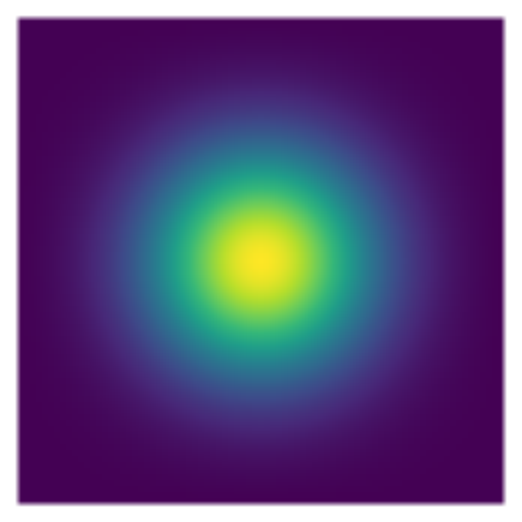
\includegraphics[width=\linewidth]{fig_harmonic2d_net.png}
  \caption{harmonic, network}
\end{subfigure}\hfill
\begin{subfigure}{0.31\linewidth}
  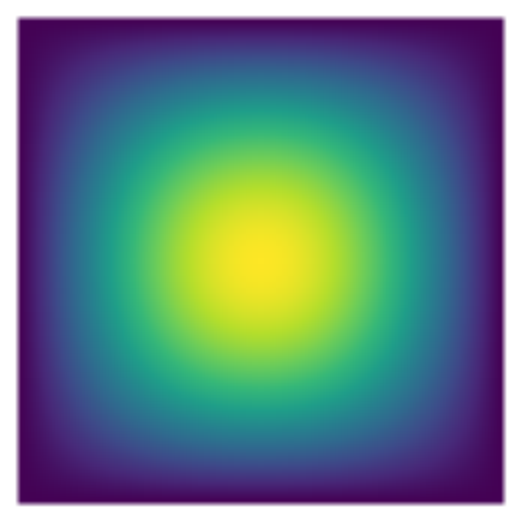
\includegraphics[width=\linewidth]{fig_well2d_net.png}
  \caption{box, network}
\end{subfigure}\hfill
\begin{subfigure}{0.31\linewidth}
  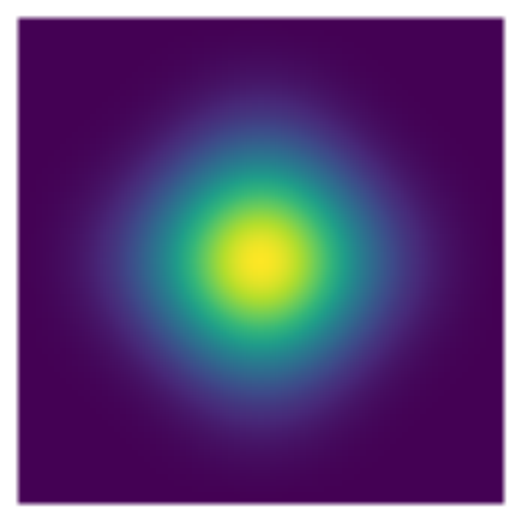
\includegraphics[width=\linewidth]{fig_anharmonic2d_net.png}
  \caption{anharmonic, network}
\end{subfigure}

\vspace{2pt}
\begin{subfigure}{0.31\linewidth}
  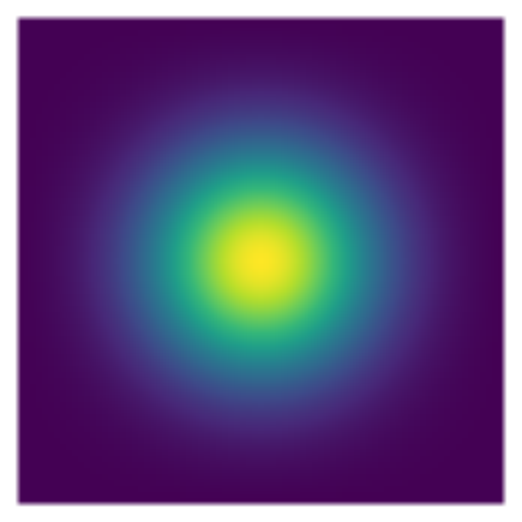
\includegraphics[width=\linewidth]{fig_harmonic2d_ref.png}
  \caption{harmonic, reference}
\end{subfigure}\hfill
\begin{subfigure}{0.31\linewidth}
  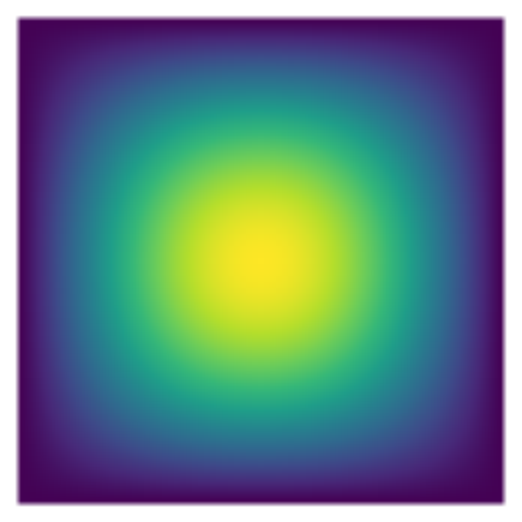
\includegraphics[width=\linewidth]{fig_well2d_ref.png}
  \caption{box, reference}
\end{subfigure}\hfill
\begin{subfigure}{0.31\linewidth}
  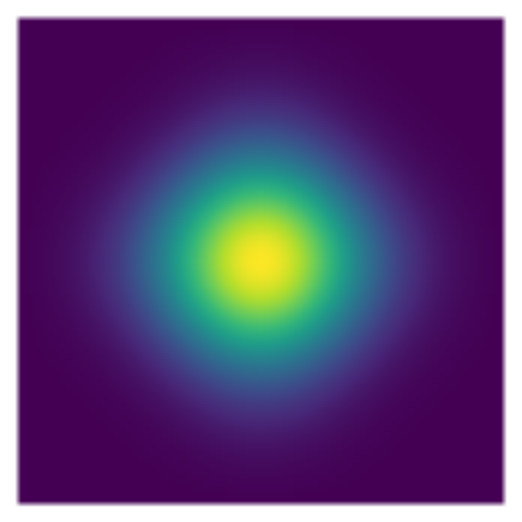
\includegraphics[width=\linewidth]{fig_anharmonic2d_ref.png}
  \caption{anharmonic, reference}
\end{subfigure}
\caption{Two-dimensional ground states: trained network (top) and discrete
reference (bottom), each normalised to its own maximum. Every reference field
is the ground eigenvector of the \emph{same} $\Hh$, returned by ARPACK on the
same grid; its eigenvalue agrees with the dense LAPACK values of
Table~\ref{tab:2d} to at least twelve digits. The reference is for display
only and enters no error estimate. Colour maps are linear in $|\psi|$.}
\label{fig:heatmaps}
\end{figure}

\subsection{Degenerate states are refused as states, certified as subspaces}
\label{sec:deg-results}

Table~\ref{tab:degeneracy} feeds \emph{exact} ARPACK eigenvectors of the box
potential into the single-state certificate. The ground state is certified with
width $2.0\times10^{-11}$. The first excited level is doubly degenerate: the
two eigenvalues differ by less than $2\times10^{-13}$ (round-off; the exact
value depends on the solver's start vector) and the eigenvectors are
$4\times10^{-12}$-accurate, yet the certificate refuses both of them and a
$0.43$ mixture.

\begin{table}[t]
\centering
\small
\setlength{\tabcolsep}{2pt}
\begin{tabular}{lccccc}
\toprule
Input state & $E$ & $r$ & certified & width & outcome \\
\midrule
Ground state & 9.868336 & $3.3\times10^{-12}$ & yes & $2.0\times10^{-11}$ & accepted \\
Excited (ARPACK 1) & 24.663232 & $4.3\times10^{-12}$ & no & -- & refused \\
Excited (ARPACK 2) & 24.663232 & $4.0\times10^{-12}$ & no & -- & refused \\
Excited (mixture) & 24.663232 & $4.8\times10^{-12}$ & no & -- & refused \\
\bottomrule
\end{tabular}

\caption{Degeneracy experiment on the $81\times81$ box. The verified gap for
the refused states is $7.1\times10^{-9}$, below the resolution floor
$1.3\times10^{-5}$ of \eqref{eq:floor}.}
\label{tab:degeneracy}
\end{table}

The refusal is the correct answer: no interval can contain exactly one of the
two eigenvalues, so neither \eqref{eq:temple} nor \eqref{eq:dk} has a
hypothesis, and the statement ``the state is identified'' is false even though
the residual is $10^{-12}$. The four rows make the point quantitatively: the residuals differ by less than
a factor of $1.5$ between the accepted ground state and the three refused
excited states, so a convention that reports residuals alone would rank them
as equally accurate, while the certificate's answer for the excited states is
that no eigenfunction is defined and nothing is certified. In a workflow that
ranks states or feeds them into a downstream calculation, that difference is
decisive.

\paragraph{The same data, certified as a subspace}
Table~\ref{tab:subspace} applies the cluster certificate of
Section~\ref{sec:subspace} to the same eigenspace. Given the two exact
eigenvectors the verified count returns $N(b)-N(a)=2$ on the interval
$(17.2658,\,32.0607)$, the Ritz residual is $\rho_F=6.1\times10^{-12}$ at the margin
$\delta=7.397$, and Theorem~\ref{thm:angle} bounds the angle to the
true invariant subspace by $8.2\times10^{-13}$, against a true angle of
$2.3\times10^{-16}$. The eigenvectors that ARPACK returns for a degenerate
level depend on its start vector, so the residual---and with it the last digit
of the bound---moves between runs ($8.2$--$8.5\times10^{-13}$); the verified
interval and the acceptance do not, and it is those that the certificate
asserts. The rotated basis $(x_1,\,0.6x_1+0.8x_2)$ returns the same
interval to all printed digits, which is the basis independence of the
symmetric orthogonalization; the certificate depends on $\operatorname{span}$
and not on how the columns were chosen. The refusals are equally
informative: one member of the pair alone ($m=1$) is refused because no
interval isolates it, and the set $\{\text{ground},\ \text{4th level}\}$ is
refused because any interval containing both of its Ritz values also
contains the degenerate pair, so the count is $4$, not $2$.
A subspace that skips a state is never reported as a smaller success.

\begin{table}[t]
\centering
\scriptsize
\setlength{\tabcolsep}{2pt}
\begin{tabular}{lccccccc}
\toprule
Input & $m$ & $N(b)\!-\!N(a)$ & $\rho_F$ & $\delta$ & $\Theta\le$ & $\Theta_{\mathrm{true}}$ & outcome \\
\midrule
Exact pair & 2 & 2 & $6.1\times10^{-12}$ & $7.4$ & $8.2\times10^{-13}$ & $2.3\times10^{-16}$ & accepted \\
Exact pair, rotated basis & 2 & 2 & $6.3\times10^{-12}$ & $7.4$ & $8.5\times10^{-13}$ & $3.0\times10^{-16}$ & accepted \\
One member ($m=1$) & 1 & -- & $4.4\times10^{-12}$ & -- & -- & -- & refused \\
Ground $+$ 4th level & 2 & -- & $5.7\times10^{-12}$ & -- & -- & -- & refused \\
\midrule
Networks 0, 1 & 2 & -- & $16.3$ & $6.08$ & -- & -- & refused \\
Networks 0, 2 & 2 & 2 & $4.6$ & $7.31$ & $0.68$ & $2.8\times10^{-2}$ & accepted \\
Networks 0, 3 & 2 & 2 & $4.1\times10^{-2}$ & $7.4$ & $5.6\times10^{-3}$ & $3.0\times10^{-4}$ & accepted \\
Networks 1, 2 & 2 & -- & $7.53$ & $7.18$ & -- & -- & refused \\
Networks 1, 3 & 2 & 2 & $4.5\times10^{-2}$ & $7.4$ & $6.1\times10^{-3}$ & $2.4\times10^{-4}$ & accepted \\
Networks 2, 3 & 2 & 2 & $4.7\times10^{-2}$ & $7.4$ & $6.3\times10^{-3}$ & $2.5\times10^{-4}$ & accepted \\
Seeds 0, 1, rotated & 2 & -- & $16.3$ & $6.08$ & -- & -- & refused \\
Seeds 0, 3, rotated & 2 & 2 & $4.1\times10^{-2}$ & $7.4$ & $5.6\times10^{-3}$ & $3.0\times10^{-4}$ & accepted \\
Network $+$ partner & 2 & 2 & $3.8\times10^{-2}$ & $7.4$ & $5.2\times10^{-3}$ & $2.8\times10^{-4}$ & accepted \\
Network $+$ mix, partner & 2 & 2 & $3.8\times10^{-2}$ & $7.4$ & $5.2\times10^{-3}$ & $2.8\times10^{-4}$ & accepted \\
\bottomrule
\end{tabular}

\caption{Cluster certificates on the $81\times81$ box. $m$ is the number of
vectors supplied, $N(b)-N(a)$ the \emph{verified} multiplicity (a dash when the
certificate refuses before the count is meaningful), $\rho_F$ the Frobenius
residual, $\delta$ the cluster margin \eqref{eq:margin}, $\Theta$ the
certified angle bound $\arcsin(\rho_F/\delta)$ and $\Theta_{\mathrm{true}}$ the
true principal angle, both in radians and the latter computed with a dense
reference. In the neural block,
runs 0, 1 and 2 converged to the same representative and run 3 to its partner;
the certificate accepts the pairs that contain run 3, refuses $(0,1)$ and
$(1,2)$, and accepts $(0,2)$ with a much weaker bound. The last two rows use a
direction forced by deflating the first output.}
\label{tab:subspace}
\end{table}

\paragraph{Where the boundary lies: resolution, not degeneracy}
Table~\ref{tab:resolution} replaces the question ``is this level degenerate?''
by a measurement. Adding the anisotropy $\lambda(x^2-y^2)$ to the box splits
the pair by $0.076\,\lambda$ with the mean energy unchanged to the printed
digits, and the certificate is applied to both members at thirteen values of
$\lambda$. The single-state certificate refuses every pair whose splitting
lies below the counting floor---including splittings of $10^{-7}$ and
$10^{-6}$, six orders of magnitude above round-off and separated by ARPACK
without difficulty---and accepts as soon as the splitting passes it: refused
at $\text{split}/\text{floor}=0.95$, accepted at $1.01$, a factor of $1.06$
between the two. The quantity compared with the floor is the verified gap,
and its value is set by the interval construction. Above the transition the
endpoints sit a tenth of the splitting inside each neighbour, so the gap is
$0.9\times$split; at the crossing that proposal cannot clear the floor, the
count-bisection fallback returns an endpoint at the neighbouring eigenvalue,
and the gap is the splitting itself---which is why acceptance begins exactly
at $\text{split}/\text{floor}=1$ rather than at $1/0.9$. The cluster
certificate, by contrast, accepts at every $\lambda$, exact degeneracy
included, with the same margin $\delta=7.397$ and a bound of
$7.4$--$9.8\times10^{-13}$: its margin is the distance to the next level, not
the internal splitting.

The practical content is that the phrase ``degenerate state'' is the wrong
category for this protocol. What decides certifiability is whether two shifts
can be separated in floating point, and a level split by $10^{-6}$ is as
uncertifiable as one split by $10^{-13}$. A practitioner who reports a pair of
near-degenerate states separately, with a validated interval each, cannot
support that claim on this grid; the pair as a subspace is certified to
$8\times10^{-13}$ in the same run.

\begin{table}[t]
\centering
\footnotesize
\setlength{\tabcolsep}{2pt}
\begin{tabular}{lcccccc}
\toprule
$\lambda$ & split $|E_1-E_2|$ & floor & split/floor & single state & $\delta$ & $\Theta\le$ \\
\midrule
$0$ & $<10^{-12}$ & $1.3\times10^{-5}$ & $<0.01$ & refused & $7.4$ & $8.4\times10^{-13}$ \\
$1.0\times10^{-5}$ & $7.6\times10^{-7}$ & $1.3\times10^{-5}$ & $0.06$ & refused & $7.4$ & $7.5\times10^{-13}$ \\
$3.0\times10^{-5}$ & $2.3\times10^{-6}$ & $1.3\times10^{-5}$ & $0.18$ & refused & $7.4$ & $8.7\times10^{-13}$ \\
$1.0\times10^{-4}$ & $7.6\times10^{-6}$ & $1.3\times10^{-5}$ & $0.59$ & refused & $7.4$ & $8.1\times10^{-13}$ \\
$1.5\times10^{-4}$ & $1.1\times10^{-5}$ & $1.3\times10^{-5}$ & $0.89$ & refused & $7.4$ & $7.6\times10^{-13}$ \\
$1.6\times10^{-4}$ & $1.2\times10^{-5}$ & $1.3\times10^{-5}$ & $0.95$ & refused & $7.4$ & $7.6\times10^{-13}$ \\
$1.7\times10^{-4}$ & $1.3\times10^{-5}$ & $1.3\times10^{-5}$ & $1.01$ & accepted & $7.4$ & $8.1\times10^{-13}$ \\
$1.9\times10^{-4}$ & $1.4\times10^{-5}$ & $1.3\times10^{-5}$ & $1.13$ & accepted & $7.4$ & $7.6\times10^{-13}$ \\
$2.0\times10^{-4}$ & $1.5\times10^{-5}$ & $1.3\times10^{-5}$ & $1.19$ & accepted & $7.4$ & $7.4\times10^{-13}$ \\
$3.0\times10^{-4}$ & $2.3\times10^{-5}$ & $1.3\times10^{-5}$ & $1.78$ & accepted & $7.4$ & $7.7\times10^{-13}$ \\
$4.0\times10^{-4}$ & $3.0\times10^{-5}$ & $1.3\times10^{-5}$ & $2.37$ & accepted & $7.4$ & $9.8\times10^{-13}$ \\
$1.0\times10^{-3}$ & $7.6\times10^{-5}$ & $1.3\times10^{-5}$ & $5.94$ & accepted & $7.4$ & $8.3\times10^{-13}$ \\
$1.0\times10^{-2}$ & $7.6\times10^{-4}$ & $1.3\times10^{-5}$ & $59.37$ & accepted & $7.4$ & $8.2\times10^{-13}$ \\
\bottomrule
\end{tabular}

\caption{Resolution boundary on the $81\times81$ box perturbed by
$\lambda(x^2-y^2)$, which splits the level linearly with the mean energy
unchanged. ``floor'' is $10^{-9}s$ of \eqref{eq:floor}. The single-state
certificate accepts when the verified gap passes the floor; the gap is nine
tenths of the splitting above the transition and equal to it at the crossing,
so acceptance begins at $\text{split}/\text{floor}\approx1$. The cluster
certificate has no such transition. Widths are
omitted because the two-sided enclosure of an exact eigenvector is at the
round-off floor ($4.9\times10^{-11}$) in every accepted row.}
\label{tab:resolution}
\end{table}

\paragraph{Independent runs: which sets span the level?}
Four additional runs, initialised differently and each deflated against the
certified ground state, all reach the excited level: their energies agree with
the discrete eigenvalue $24.663232$ to $4.1\times10^{-6}$, their residuals lie
in $2.7$--$3.4\times10^{-2}$, every one is refused by the single-state
certificate (verified gap $3.8$--$4.1\times10^{-6}$, below the counting floor),
and every one lies in the exact eigenspace (fraction of its norm
$\ge0.99999996$). They are nevertheless not four independent directions. Runs
0, 1 and 2 converged to the same representative---pairwise overlaps
$0.99996$--$0.999997$, mutual angles $0.14^\circ$--$0.52^\circ$---while run 3
converged to the orthogonal partner, with overlap $0.01$ with the others.
Whether a set of runs spans the level is therefore an empirical question with
no structural answer, and the certificate answers it for each set from the
vectors alone:
\begin{itemize}
\item $(0,1)$ is refused. The two outputs differ by $2.4\times10^{-3}$ in
  $L^2$, so the only second direction in their span is that difference, at
  grid scale; its Ritz residual is $16.25$, far above the margin $6.08$, and
  Lemma~\ref{lem:cluster} has no hypothesis to stand on. $(1,2)$ is refused
  for the same reason, at $\rho_F=7.53$ and $\delta=7.18$.
\item $(0,2)$ is accepted, but weakly: $\rho_F=4.60$ gives the bound $0.68$
  against a true angle of $0.028$. The certificate cannot know that this
  second direction is mostly noise; it can only report that the bound is two orders of
  magnitude looser than for a genuine pair---and it is still a valid bound.
\item $(0,3)$, $(1,3)$ and $(2,3)$ are accepted with
  $\rho_F=4.1$--$4.7\times10^{-2}$, $\delta=7.397$ and bounds
  $5.6$--$6.3\times10^{-3}$ against true angles of
  $2.4$--$3.0\times10^{-4}$.
\end{itemize}
No energy or residual separates these cases: the energies agree to
$4\times10^{-6}$ and the residuals lie in the same narrow band. Only the
subspace certificate does, and it orders the evidence the way a reader would.
Figure~\ref{fig:deg} shows the four functions behind the table: the two
symmetry-related representatives that the runs converged to, next to the two
exact modes they approximate.

\paragraph{A forced second direction}
When the goal is to certify the level rather than to test whether training
explored it, the second direction can be forced. Deflating the first network
output in addition to the ground state---the same projection that is applied
inside the loss---produces a function orthogonal to both (overlap
$10^{-18}$ with the first output), which still lies in the level:
$0.99999997$ of its norm is in the exact eigenspace, and it coincides with the
partner that run~3 found independently (overlap $0.99995$). The pair is
accepted with verified multiplicity $2$, $\rho_F=3.8\times10^{-2}$,
$\delta=7.397$ and an angle bound of $5.2\times10^{-3}$ against a true
principal angle of $2.8\times10^{-4}$. Rotating the basis
($0.6\psi_0+0.8\psi_\perp$ in place of $\psi_\perp$) leaves the interval, the
multiplicity and the bound unchanged, as it must: the object certified is the
subspace.

\begin{figure}[t]
\centering
\begin{subfigure}{0.24\linewidth}
  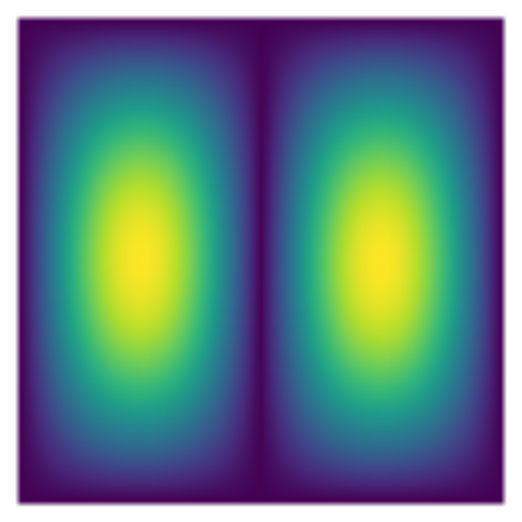
\includegraphics[width=\linewidth]{fig_deg_net_a.png}
  \caption{network, seed 0}
\end{subfigure}\hfill
\begin{subfigure}{0.24\linewidth}
  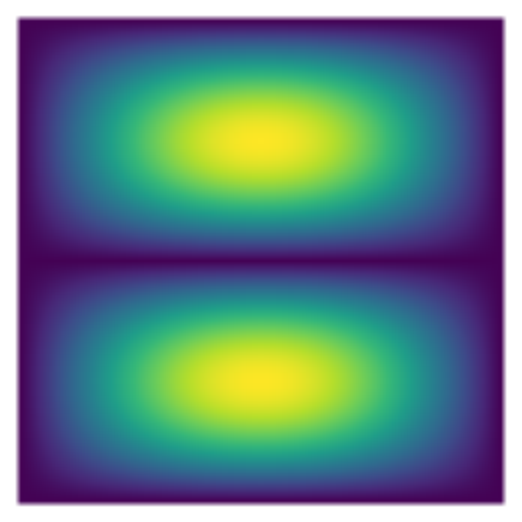
\includegraphics[width=\linewidth]{fig_deg_net_b.png}
  \caption{network, seed 3}
\end{subfigure}\hfill
\begin{subfigure}{0.24\linewidth}
  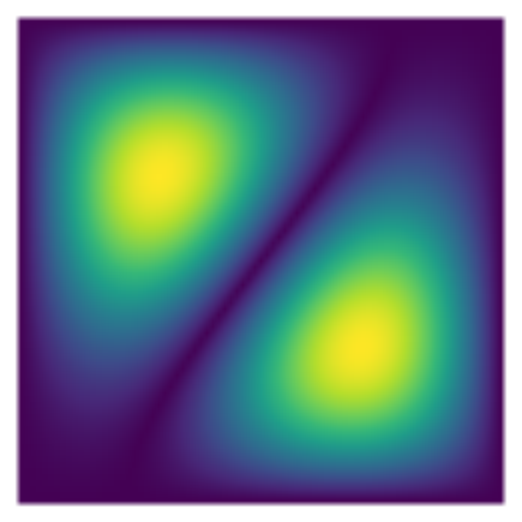
\includegraphics[width=\linewidth]{fig_deg_exact_a.png}
  \caption{exact, $\sin\pi x\sin2\pi y$}
\end{subfigure}\hfill
\begin{subfigure}{0.24\linewidth}
  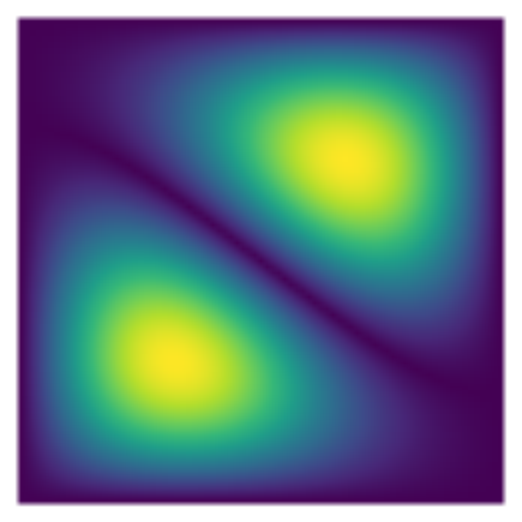
\includegraphics[width=\linewidth]{fig_deg_exact_b.png}
  \caption{exact, $\sin2\pi x\sin\pi y$}
\end{subfigure}
\caption{The doubly degenerate first excited level of the box, $|\psi|$ on the
$81\times81$ grid, each panel normalised to its own maximum. The two network
outputs are independent runs against the deflated ground state: one collapsed
onto the representative found by three of the four runs, the other onto its
orthogonal partner. They are visibly different functions---the nodal lines of
one are the reflections of the other's---and they span the same eigenspace to
within the certified angle.}
\label{fig:deg}
\end{figure}

The practical lesson is not that degenerate states are hard to train: all
four runs reached the level to $4\times10^{-6}$ in energy, and any of them
would pass a residual-based test. It is that the quantities such a run
reports---residual, energy, overlap with a chosen reference---are basis
dependent at a degenerate level, and that whether a set of outputs spans the
level is visible in none of them. The cluster certificate makes that question
decidable: it accepts the spanning pairs with a bound, refuses the collapsed
pair with a reason, and prices the difference between them in the bound
itself. A degenerate level can therefore be certified without a reference
solution, provided the dimension of the trial subspace is measured rather than
assumed.

\subsection{The discretization gap}
\label{sec:discretization}

Because the certificate refers to $\Hh$, its width bounds the error against
the discrete eigenvalue only; the distance to the continuous eigenvalue is a
separate quantity, bounded from above by the variational principle of
Section~\ref{sec:variational} and tabulated there. The two are independent:
the box width below is $2\times10^{-11}$ while the discretization error at the
same grid is $1.3\times10^{-3}$. Table~\ref{tab:disc}
quantifies that distance for the two potentials whose truncated-domain
eigenvalue can be extrapolated, using verified count bisection at five grids;
the extrapolated value $\lambda^\ast$ agrees with the variational bracket of
Table~\ref{tab:continuous} at the corresponding grid, which is the check that
the two independently computed descriptions of the same gap are consistent.

\begin{table}[t]
\centering
\small
\footnotesize
\setlength{\tabcolsep}{2.5pt}
\begin{tabular}{lcccccc}
\toprule
Pot.\ & $41$ & $61$ & $81$ & $101$ & $121$ & $\lambda^\ast$ \\
\midrule
Harmonic (2D) & $1.4\times10^{-3}$ & $6.2\times10^{-4}$ & $3.5\times10^{-4}$ & $2.2\times10^{-4}$ & $1.5\times10^{-4}$ & 1.0007826 \\
Box (2D) & $5.1\times10^{-3}$ & $2.3\times10^{-3}$ & $1.3\times10^{-3}$ & $8.1\times10^{-4}$ & $5.6\times10^{-4}$ & 9.8696042 \\
\bottomrule
\end{tabular}

\caption{Discretization error $|\lambda_h-\lambda^\ast|$ of the first
eigenvalue of $\Hh$; column headers are the grid size $N$ and
$\lambda^\ast$ is fitted from $\lambda(h)=\lambda^\ast+ch^2$. The
least-squares slope of $\log|\lambda_h-\lambda^\ast|$ against $\log h$ is
$2.00$ for both potentials.}
\label{tab:disc}
\end{table}

Two features deserve comment. The box potential extrapolates to
$\lambda^\ast=9.8696042046$, within $2.0\times10^{-7}$ of $\pi^2$, with a
clean second-order convergence; this is an end-to-end check of the counting,
bisection and extrapolation chain. The harmonic potential is subtler: its
infinite-domain eigenvalue is $1$, but the Dirichlet problem on the truncated
box $[-3,3]^2$ has eigenvalue $\lambda^\ast=1.0007826$, higher by
$7.8\times10^{-4}$ because the Gaussian tail is cut off. Consequently the raw
error against the analytic value $1$ \emph{increases} with $N$
($1.7\times10^{-4}$ at $N=61$ to $6.3\times10^{-4}$ at $N=121$) while the true
discretization error decreases at second order. Reporting only the first
column would look like a bug; reporting only the second would hide the
truncation. Both are needed, and the certificate makes the distinction
unavoidable.

At $N=81$ the harmonic discretization error against $\lambda^\ast$ is
$3.5\times10^{-4}$, three to eight times larger than the certified width of
the trained network ($0.5$--$1.1\times10^{-4}$). On this grid the network is
already better than the grid, and the certificate correctly reports the grid's
limitation rather than the network's.

\subsection{How tight is the enclosure?}
\label{sec:tightness}

Figure~\ref{fig:scatter} plots the certified width against the true error for
all 18 runs, together with the lines width $=10^{k}\times$ error. Across the
whole set the certified width lies between $5$ and $3\times10^{3}$ times the
true error, with a median ratio of $45$ over all 18 runs ($1.4\times10^{2}$
over the nine one-dimensional runs, $34$ over the two-dimensional ones). The
spread follows the potential rather than the dimension: $5$--$36$ on the
harmonic and anharmonic problems, $50$--$3\times10^{2}$ on the infinite well,
and $7\times10^{2}$--$3\times10^{3}$ on the finite well and the box. The two
large groups are large for different reasons. On the infinite well and the box
both the width and the error have reached the round-off floor
($9.9\times10^{-12}$ against $10^{-13}$ in one dimension, $2.0\times10^{-11}$
against $2.5\times10^{-14}$ in two), so the ratio is a ratio of round-off and
says nothing about the method; on the finite well neither quantity is at
round-off and the enclosure is genuinely wide, because the residual cannot
distinguish a high-wavenumber error from a genuine component of the same shape
(Section~\ref{sec:discussion}). For comparison, the same certificate applied to a
classical LAPACK eigenvector of the same $\Hh$ gives widths of
$2.0\times10^{-12}$ (harmonic), $9.9\times10^{-12}$ (infinite well) and
$9.8\times10^{-11}$ (finite well), saved by
\texttt{scripts/lapack\_reference\_widths.py} in
\url{runs/reference1d/lapack_certificates.json}: the machinery itself is not the limitation,
and a trained network's certified width is seven to ten orders of magnitude
wider on the harmonic and finite-well potentials. The infinite well is the
exception that proves the rule---after filtering, the network output is a
single sine mode, so its certificate sits at the same round-off floor as the
classical eigenvector's.

\begin{figure}[t]
\centering
\begin{tikzpicture}
\begin{axis}[
  width=0.62\linewidth, height=0.55\linewidth,
  xmode=log, ymode=log,
  xlabel={$|E_f-\lambda_h|$}, ylabel={certified width},
  xmin=1e-14, xmax=1e-2, ymin=1e-13, ymax=1e1,
  legend style={font=\footnotesize, at={(0.02,0.98)}, anchor=north west},
  grid=major, grid style={gray!25},
]
\addplot[only marks, mark=*, mark size=1.6pt, blue]
  table[col sep=comma,x=dE,y=width] {figures/data/scatter_1D_harmonic.csv};
\addplot[only marks, mark=square*, mark size=1.6pt, red!70!black]
  table[col sep=comma,x=dE,y=width] {figures/data/scatter_1D_finite_well.csv};
\addplot[only marks, mark=triangle*, mark size=2.2pt, green!50!black]
  table[col sep=comma,x=dE,y=width] {figures/data/scatter_1D_infinite_well.csv};
\addplot[only marks, mark=diamond*, mark size=2.2pt, orange!80!black]
  table[col sep=comma,x=dE,y=width] {figures/data/scatter_2D_harmonic2d.csv};
\addplot[only marks, mark=pentagon*, mark size=2.2pt, purple]
  table[col sep=comma,x=dE,y=width] {figures/data/scatter_2D_anharmonic2d.csv};
\addplot[only marks, mark=o, mark size=2.2pt, cyan!70!black]
  table[col sep=comma,x=dE,y=width] {figures/data/scatter_2D_well2d.csv};
\addplot[domain=1e-14:1e-2, dashed, black!60] {x};
\addplot[domain=1e-14:1e-4, dashed, black!35] {100*x};
\addplot[domain=1e-14:1e-6, dashed, black!20, forget plot] {10000*x};
\legend{1D harmonic, 1D finite well, 1D infinite well,
        2D harmonic, 2D anharmonic, 2D box}
\end{axis}
\end{tikzpicture}
\caption{Certified width against true error. Dashed lines: width $=$ error,
$100\times$ error, $10^4\times$ error. The points at the far left are the
infinite-well and box runs, whose filtered states are exact sine modes; the
upper-right outliers are the finite well.}
\label{fig:scatter}
\end{figure}

The figure also shows where the enclosure is genuinely informative: for the
smooth harmonic and anharmonic potentials the ratio is $5$--$40$, which is
enough to certify that a network is accurate to, say, $10^{-4}$ without any
reference. For the finite well the ratio is $10^{3}$ and only the
containment statement survives.

\begin{figure}[t]
\centering
\begin{subfigure}{0.48\linewidth}
\begin{tikzpicture}
\begin{axis}[
  width=0.94\linewidth, height=0.78\linewidth,
  xmode=log, ymode=log,
  xlabel={cutoff $K$}, ylabel={certified width},
  legend style={font=\scriptsize, at={(0.02,0.98)}, anchor=north west},
  grid=major, grid style={gray!25},
]
\addplot[thick, blue, mark=*, mark size=1pt]
  table[col sep=comma,x=cutoff,y=width] {figures/data/width_vs_cutoff_harmonic.csv};
\addplot[thick, red!70!black, mark=square*, mark size=1pt]
  table[col sep=comma,x=cutoff,y=width] {figures/data/width_vs_cutoff_finite_well.csv};
\addplot[thick, green!50!black, mark=triangle*, mark size=1pt]
  table[col sep=comma,x=cutoff,y=width] {figures/data/width_vs_cutoff_infinite_well.csv};
\legend{harmonic, finite well, infinite well}
\end{axis}
\end{tikzpicture}
\caption{width vs.\ truncation order}
\end{subfigure}\hfill
\begin{subfigure}{0.48\linewidth}
\begin{tikzpicture}
\begin{axis}[
  width=0.94\linewidth, height=0.78\linewidth,
  xmode=log, ymode=log,
  xlabel={$h$}, ylabel={$|\lambda_h-\lambda^\ast|$},
  legend style={font=\scriptsize, at={(0.5,0.03)}, anchor=south},
  grid=major, grid style={gray!25},
]
\addplot[thick, blue, mark=*, mark size=1.2pt]
  table[col sep=comma,x=h,y=error] {figures/data/conv2d_harmonic2d.csv};
\addplot[thick, red!70!black, mark=square*, mark size=1.2pt]
  table[col sep=comma,x=h,y=error] {figures/data/conv2d_well2d.csv};
\addplot[dashed, black!45, domain=0.008:0.16] {8.1*x^2};
\legend{harmonic (2D), box (2D), $8.1\,h^2$}
\end{axis}
\end{tikzpicture}
\caption{discretization error vs $h$}
\end{subfigure}
\caption{(a) Certified width against the DST truncation order for one run
per potential; the minimum is what the protocol selects
without a reference. (b) Discretization error of the two-dimensional ground
states against the $h\to0$ limit; the dashed line is the expected second-order
slope.}
\label{fig:filter}
\end{figure}

\section{Discussion}
\label{sec:discussion}

\subsection{What the protocol buys, and what it costs}

The certificate turns an approximation into a statement with a hypothesis and
a conclusion: \emph{if} the interval contains exactly one eigenvalue (checked),
\emph{then} the eigenvalue lies in $[\eta-\rho^2/(b-\eta),\,\eta+\rho^2/(\eta-a)]$
and the eigenfunction is within $\arcsin(\rho/\gamma)$ of $\psi$. The
hypothesis is the part that classical presentations leave to the user; making
it a computation is what allows the bound to be used on a mesh-free
approximation whose spectrum is unknown.

The cost is small. In two dimensions a certificate requires four to six
verified counts, each a sparse factorization taking $0.03$\,s at
$81\times81$; in one dimension a count takes $0.4$\,ms, so the count-only
bisection fallback can be used freely and a certificate spends some two
hundred of them. Measured end to end, a full certificate takes $0.19$\,s and
$0.074$\,s against $30$--$110$\,s of training. The guided filter repeats the certificate at each
candidate cutoff---$27$ candidates in the one-dimensional runs and $30$--$62$
in the two-dimensional ones---which costs $2.6$\,s and, scaled from the
measured $16$\,s at $81$ candidates, $6$--$12$\,s, still seconds. There is no reason not to certify every run that is reported.

The benefit is not accuracy but accountability. In our own experiments the
certificate changed decisions four times: it rejected an excited-state run
that had a valid-looking energy (state index mismatch), it exposed a
degenerate state masquerading as a $10^{-12}$-accurate one, it showed that
part of what looked like network error on the finite well was discretization
error that no amount of training could remove, and it decided which pairs of
independently trained networks actually span a degenerate level---accepting
the three pairs that contain the orthogonal partner with bounds of
$5$--$6\times10^{-3}$, refusing the two collapsed pairs, and pricing the
ambiguous pair at $0.68$.

\subsection{Limitations}

\paragraph{The enclosure can be uninformative} For the finite well the ratio
of certified width to true error is $10^{3}$ and the angle bound is $O(1)$.
The bound is correct and useless. This is not a defect of the implementation
but a property of residual-based bounds on non-smooth problems: the residual
cannot distinguish a genuine high-wavenumber component from an error of the
same shape, and the spectral gap at the relevant scale is large enough that
the quadratic Temple gain does not compensate. Any claim that such bounds
``certify PINN accuracy'' must be conditioned on the potential.

\paragraph{Degeneracy is now inside the protocol, but only at counting
resolution} The cluster certificate of Section~\ref{sec:subspace} removes the
structural obstacle: a degenerate level is certified as an invariant subspace,
with the multiplicity measured by the count and the angle bounded by
Theorem~\ref{thm:angle}. Two limitations remain, and they are of different
kinds. The first is the resolution floor \eqref{eq:floor}: two shifts closer
than $10^{-9}s$ cannot be separated by the count, and a cluster whose boundary
margin falls below the floor is refused---including, as the degeneracy
experiment shows, a pair that double precision can barely split. The floor is
a declared safety margin rather than a theorem (Section~\ref{sec:floor}), and
directed rounding does not remove it: it makes the count beneath the margin
exact, so that the refusal happens for a stated reason at a stated pivot,
rather than moving the margin. Counting at a higher precision would move the
floor but not abolish the need for one. The second limitation is structural: a
trial subspace that omits a member of the level is refused because its
dimension disagrees with the count, which is the correct answer but means that
the certificate can detect a wrong basis and cannot repair it. A milder
limitation is that the cluster bound is first order in $\rho$: unlike the
Kato--Temple bound it does not improve quadratically as the residual shrinks,
because a cluster has no interior eigenvalue to isolate. For very accurate
subspaces the counting resolution, not the angle bound, becomes the limiting
quantity.

\paragraph{The certified object is discrete} The gap between $\Hh$ and
$\mathcal H$ is $O(h^2)$ for smooth eigenfunctions and dominates the
certificate at the grid sizes used here (Section~\ref{sec:discretization}). A
certificate for the continuous operator would require either an explicit
$O(h^2)$ bound with computable constants, or a homotopy-based enclosure of the
elliptic problem itself \citep{plum1991}, which needs a priori pointwise
bounds on the eigenfunction that a trained network does not supply; nor is a
$p$-version/spectral discretization with exponential convergence implemented.
We do not claim any of the three. What
Section~\ref{sec:variational} does claim is the one-sided half, and it is
enough to change what a reported energy means: the interpolant of the network
eigenfunction is a conforming trial function, so its Rayleigh quotient bounds
the continuous eigenvalue from above without any regularity input. The other
side is where the difficulty sits, and the finite well shows it is not a
technicality: a certified discrete eigenvalue can lie \emph{above} the
continuous one when the potential is discontinuous, so no care with the
factorization turns a discrete count into a continuous enclosure. The same boundary explains why the count
refers to $\Hh$ and not to the spectrum of a non-conforming trial space: such
a space can carry spurious eigenvalues \citep{lewinsere2010}, so a discrete
eigenvalue computed from it would not by itself identify the state it belongs
to.

\paragraph{Directed rounding in one dimension, not in general two} The count
of Section~\ref{sec:certified} is computed with outward rounding, so in one
dimension---and in two whenever the potential is separable, which covers the
harmonic oscillator and the box---it is a theorem about the stored matrix
rather than a guarded estimate. What remains outside is the general
two-dimensional count for a non-separable potential: the interval elimination
refuses on most shifts at the grid sizes we use, so the anharmonic experiments
still read their count off the floating-point factorization with the checks of
Section~\ref{sec:counting}. We report that measurement rather than route
around it. The separable construction suggests the next step---splitting a
non-separable potential into separable pieces and carrying the remainder as a
perturbation---but we have not implemented it, and we do not claim it here.

\paragraph{Statistical power} We report counts, not rates with confidence
intervals. Every enclosure we report contains the discrete eigenvalue to which
it refers---the eighteen of the main sweep, the nine learnable-energy and nine
reference-energy runs of the leakage audit, and the three deflated runs, for
$39/39$; in the multi-state chain each enclosure contains the eigenvalue of
the state that its certified index names. The Wilson 95\% interval for
$39/39$ is $[0.91,1.0]$, so the data are
still consistent with a per-run failure probability as large as $9\%$; the
eighteen runs of the main sweep alone give $[0.82,1.0]$. The multi-state chain
is the more demanding test and is not perfect: $25/27$ certify the
\emph{requested} state, Wilson $[0.77,0.98]$, with both failures traced to an
upstream state mismatch that the state index flagged. A claim of the form
``the method certifies correctly with probability at least $0.95$'' would
require about seventy runs with no failure, and we do not make it.

\subsection{Why not solve \texorpdfstring{$\Hh$}{H\_h} instead?}
\label{sec:why}

A referee may reasonably ask what the certificate adds, since on every
problem in this paper $\Hh$ is assembled and a shift-invert Lanczos solve of
the same matrix returns $\lambda_h$ and its eigenvector in $20$\,ms at
$81\times81$ and $1.7$\,ms at $N=2001$, roughly ten times faster than the
certificate in two dimensions and forty times in one ($0.19$\,s and
$0.074$\,s; both measured in
\texttt{scripts/bench\_count.py}). We do not think the answer is speed, and
the protocol should not be sold on it. Three things are at stake that a solve of $\Hh$
does not supply.

\emph{The certificate does not need a converged eigenvector.} Counting is the
only operation it performs on $\Hh$, and ARPACK is used to propose intervals
that a count then verifies; the count-only fallback of
Section~\ref{sec:isolating} removes even that. The statement therefore
attaches to the object the user has---one network output, one snapshot, one
subspace---rather than to the object a solver would produce instead.

\emph{At a degenerate level the classical comparison is ill-posed.} The
eigenvector a solver returns for a multiple eigenvalue is an arbitrary element
of the level, chosen by its tie-breaking; the overlap of the same network
output with it can be $1$ or $0$ without anything about the network
changing. The experiments of Section~\ref{sec:deg-results} are exactly this
case: three runs and the solver's eigenvector coincide, the fourth does not,
and every residual-based comparison is silent. The cluster certificate is
invariant under the choice, and it prices the difference. This is the one
place where the certificate states something that \emph{cannot} be read off a
solver's output.

\emph{The audit is of the procedure, not of a number.} State index, two-sided
enclosure, angle bound and measured multiplicity together describe a pipeline
end to end; a comparison with a reference eigenvalue describes one run. The
leakage audit (Section~\ref{sec:leak-results}) and the state-index failures of
the multi-state chain (Section~\ref{sec:multistate}) are decisions of the
first kind. This is also the honest limit of the present work: when $\Hh$
cannot be assembled---the high-dimensional regime that motivates neural
eigen-solvers in the first place---every statement here refers to a matrix
that does not exist, and matrix-free verification is open. The protocol is
addressed to the intermediate regime in which the problem is small enough to
assemble and large enough that the learned function, not the solver, is what
is being reported.

\subsection{Relation to existing work}

Enclosure of eigenvalues by variational bounds plus a verified count is the
standard toolkit of a posteriori eigenvalue analysis for finite elements
\citep{babuska1991}: the Temple and Lehmann--Goerisch bounds are used exactly
as here, and the count is usually obtained from a Cholesky factorization of
the stiffness matrix at a shift. Our contribution is not to that theory but to
its transfer: the approximation is a network, the matrix is assembled for the
certificate alone, and the two failure modes that matter in this setting
(degeneracy and leakage) are given explicit treatments.

For clusters the closest antecedent is \citet{cances2020}, who give
guaranteed two-sided bounds for eigenvalue clusters of conforming
discretizations, multiplicities included. Their analysis is built on the
Galerkin structure---residual estimators, orthogonality, and a comparison
between the approximation space and its neighbourhood. A trained network has
none of these properties, and applying those bounds to one would require
proving an analogue from scratch.
The counting route taken here needs no such hypothesis: it measures the
multiplicity directly and bounds the subspace by the residual-to-margin
ratio, which is why the same statement covers exact, approximate and
accidentally degenerate clusters.

For forward PDEs, a posteriori error estimates for physics-informed networks
have begun to appear \citep{mishra2023}; they bound the error of a solution
operator in a norm, and require regularity assumptions on the data. An
eigenvalue problem differs in that the object to be bounded is a spectral
quantity and the unknown is defined only up to a subspace; the counting
machinery is what replaces the coercivity argument.

Verified-computing libraries such as INTLAB~\citep{rump1999} and
Arb~\citep{johansson2017}, and their Python interfaces, would supply the same
arithmetic at arbitrary precision. We use only IEEE doubles with one-ulp
outward padding (\texttt{nextafter}) because the recurrences need nothing
more: the certified count is a sign test on pivots whose intervals close under
a correctly rounded operation, and the failure mode---a pivot interval that
contains zero---is detected and refused rather than hidden. The same libraries
remain the natural route to a fully rigorous two-dimensional count and to
interval enclosures of the Rayleigh quotients themselves, at a modest
constant-factor cost.

\subsection{A reporting checklist}

The experiments suggest a short checklist for papers that report neural
eigenpairs, each item of which would have changed the interpretation of at
least one run in this study:
\begin{enumerate}
\item state the discrete operator and the grid; report the discretization gap
  separately from the network error;
\item report the certified state index, not only the energy;
\item report the enclosure width, and the ratio of width to true error, not
  only the true error;
\item report raw and filtered quantities side by side, with the $L^2$ change
  caused by the filter;
\item state whether any reference quantity entered the training objective;
\item refuse to certify a degenerate state individually rather than reporting
  its residual as an accuracy, and certify the invariant subspace instead,
  with the multiplicity measured by counting.
\end{enumerate}
Items 2, 3 and 6 are cheap; they require no additional theory and would make
the reported numbers comparable across papers.

\section{Conclusion}
\label{sec:conclusion}

We have described a protocol that makes classical a posteriori eigenvalue
bounds computable for neural eigenpairs of the discrete Schr\"odinger
operator, and an implementation of it that runs on ordinary hardware. The
essential element is not any of the inequalities---they are textbook---but the
verification of their hypothesis: by counting the spectrum below two shifts
with Sturm sequences or Sylvester inertia, the interval that the theorems
require is constructed and checked rather than assumed. The same machinery
supplies the spectral gap that turns a residual into a two-sided eigenvalue
enclosure and an eigenfunction angle bound. At a degenerate level the same
machinery is applied to the invariant subspace rather than to a state: the
multiplicity is measured by the count, the cluster receives a two-sided
enclosure, and the angle between the trial subspace and the true one is
bounded, so that the structural obstacle of degeneracy becomes a certificate
rather than a refusal.

The experiments on six potentials in one and two dimensions give a concrete
picture of what can and cannot be certified. All 39 filtered enclosures we
report contain the discrete eigenvalue they refer to---18 from the main sweep
and 21 from the leakage audit, the two-dimensional ones checked against a
dense LAPACK solve rather than the ARPACK values that propose the
intervals---and the certified width is
between $5$ and $40$ times the true error on the harmonic and anharmonic
potentials, between $50$ and $3\times10^{2}$ times on the infinite well and
$7$--$8\times10^{2}$ on the box---where width and error are both at
round-off---and up to $3\times10^{3}$ times on the finite well, where the
bound is correct but uninformative. A
degenerate state with a $4\times10^{-12}$ residual is refused as a state while
the same eigenspace is accepted as a two-dimensional invariant subspace, with a
measured multiplicity of two and a principal-angle bound of
$8\times10^{-13}$ on exact inputs and $6\times10^{-3}$ on network inputs. Of
four independently trained networks on that level, three collapsed onto the
same representative and one found its partner; the certificate refused the
pairs that do not span the level and accepted the pairs that do. Splitting the
level by a controlled anisotropy locates the boundary between the two
certificates exactly at the counting resolution---a split of $10^{-6}$ is
refused as a state just as a split of $10^{-13}$ is, while the subspace is
certified in both cases---so the obstacle is computable rather than
structural. The network
error on the $81\times81$ grid is smaller than the discretization gap, so the
certificate correctly reports the grid as the limiting factor.

The implementation, the drivers that regenerate every table, and the test
suite that locks the guards are available with this article. The two open
items of the previous version of this work are closed here in part. The count
is now computed in directed-rounding interval arithmetic---provably in one
dimension, and in two dimensions whenever the potential is separable, which
covers two of our three two-dimensional problems; the general sparse
factorization still refuses too often in intervals to be useful, and we
report the measurement rather than hide it. And the continuous operator now
receives an upper bound from the variational principle---exact in exact
arithmetic, and limited only by the floating-point evaluation of the
quotient---at the price of a Rayleigh quotient rather than of an interpolation
constant; the lower
side exists only where a comparison principle does, which we demonstrate for
the infinite well and the box and show to fail for the finite well. Neither addition changes the
protocol, and neither touches the cluster construction: what limits the
certificate at a degenerate level is the resolution at which two shifts can
be separated, not the requirement that the level be simple.


\section*{CRediT authorship contribution statement}
\textbf{Chunyang Chen:} Conceptualization, Methodology, Software, Validation,
Formal analysis, Investigation, Writing -- original draft. \textbf{Yuhao
Peng:} Conceptualization, Methodology, Software, Validation, Formal analysis,
Investigation, Writing -- review and editing, Supervision. Both authors
contributed equally to this work and approved the final manuscript.

\section*{Code availability}
The implementation, the experiment drivers and the scripts that regenerate
every table and figure of this paper are part of the repository accompanying
this article, \url{https://github.com/YuhaoPeng1103/PINN_equation} (MIT
licence). A frozen archive will be deposited in the CPC Program Library.

\section*{Data availability}
All data supporting this study are contained in the repository cited above:
the measured artefacts behind every table and figure are stored under
\texttt{runs/} as JSON, CSV and NumPy archives, and the drivers that
regenerate them are in \texttt{scripts/} and \texttt{paper/}. No other data
were generated or analysed.

\section*{Declaration of competing interest}
The authors declare that they have no known competing financial interests or
personal relationships that could have appeared to influence the work
reported in this paper.

\section*{Funding}
This research did not receive any specific grant from funding agencies in the
public, commercial, or not-for-profit sectors.

\section*{Declaration of generative AI and AI-assisted technologies in the
manuscript preparation process}
During the preparation of this work the authors used Claude (Anthropic) in
order to assist with drafting and editing the manuscript text and with the
implementation and testing of the software. After using this tool, the
authors reviewed and edited the content as needed and take full
responsibility for the content of the published article.

\appendix
\section{Implementation notes}
\label{app:impl}

\subsection{Training failures that shaped the implementation}
\label{app:failures}

Three failures were reproducible and are worth recording, because each one
produces a network that looks superficially fine but cannot be certified. The
runs behind them are kept in \url{runs/appendix_fourier2d/} and
\url{runs/appendix_failures/}; the Fourier and hard-mask runs are outputs of
\texttt{scripts/exp6\_certificate\_training\_2d.py}, the soft-boundary and
unnormalized runs of \url{scripts/appendix_failures.py}.

\paragraph{Random Fourier features in two dimensions} The one-dimensional
runs use random Fourier features \citep{tancik2020} and profit from them. In
two dimensions the same configuration (scale $2.5$) stalls: at $6000$ epochs,
on the harmonic potential whose discrete eigenvalue is $1.0004$, it reaches
$E=1.5624$ and overlap $0.877$ (the $1500$-epoch snapshot is $E=1.5636$ and
$0.877$) against $E=1.0004$ and overlap $0.99997$ for the plain MLP, and the
single-state certificate refuses the output with a residual of $1.17$
(\texttt{runs/appendix\_fourier2d/}). Each feature
$\sin/\cos(\omega_1x+\omega_2y)$ must cover a direction in the plane, and the
sample efficiency of a fixed random direction set degrades with dimension. The
2D driver therefore disables Fourier features by default. This is an empirical
configuration choice, not a claim about Fourier features in general.

\paragraph{The zero function in an unnormalized loss} If the loss is the
residual of $\psi$ itself rather than of the unit vector $\psi/\norm{\psi}$,
the zero function is a global minimum and not merely a stationary point: the
Rayleigh quotient is scale invariant, so the residual is exactly linear in
$\psi$ and $L(c\psi)=c^2L(\psi)$, whence $L(0)=0\le L(\psi)$. No term then
fixes the scale: the amplitude stays wherever the initialization put it, and
any tolerance can be met by shrinking rather than by improving the shape. In a
$3000$-epoch run at $N=41$ the field ended at
$\norm{\psi}^2=6.0\times10^{-5}$, a maximum amplitude of $1.5\times10^{-2}$ (rms
$7.5\times10^{-3}$ over the grid), with
a shape that is already accurate (overlap $1.0000$ after normalization, energy
error $1.1\times10^{-5}$). Measured on the field as returned, without
normalization, the residual norm is $2.9\times10^{-4}$ while the $L^2$
distance from the discrete ground state is $0.99$---a residual three thousand
times smaller than the error it is supposed to measure
(\texttt{scripts/residual\_vs\_error.py}). Every diagnostic
computed on the normalized field therefore looks excellent while the field
itself carries a scale that the loss does not determine, and the training loss
then measures the amplitude rather than the error.
Fixing the scale by an explicit term---the penalty $(\norm{\psi}_h^2-1)^2$ in
one dimension, division by the norm in two (equation~\eqref{eq:loss})---removes
the scale direction and excludes the zero solution; the denominator is clamped
at $10^{-30}$ to keep the gradient finite during the first steps.

\paragraph{Soft boundary penalties in two dimensions} A boundary penalty with
weight $100$ does not enforce a Dirichlet condition to anything like machine
precision, because the constrained nodes are an $O(1/N)$ fraction of the grid
while the five-point Laplacian amplifies their error by $h^{-2}$. After
$3000$ epochs at $N=41$ on the box potential the penalty leaves the residual
at $5.72$ and the energy error at $5.0\times10^{-2}$ ($E=9.9144$ against the
discrete $9.8645$), with boundary nodes carrying values up to $0.22$. The
certificate still returns \texttt{valid}---its hypotheses hold for whatever
field it is given---but the enclosure is $4.68$ wide against a true error of
$5.0\times10^{-2}$, more than five orders of magnitude looser than on a
hard-constrained field. Multiplying the network output by the mask
$M=(x-a)(b-x)(y-a)(y-b)$ enforces the boundary condition exactly and is a
statement of the problem, not of the solution; with everything else unchanged
the same configuration reaches residual $1.2\times10^{-2}$, energy error
$1.2\times10^{-6}$, enclosure width $2.0\times10^{-5}$ and angle bound
$9.0\times10^{-4}$ (\texttt{runs/appendix\_failures/}). The mask costs
expressivity near the boundary, which is irrelevant for an eigenfunction that
vanishes there.

\subsection{Interval construction}
\label{app:algorithm}

\begin{center}
\fbox{\parbox{0.93\linewidth}{\small
\textbf{Algorithm 1} Verified or refused certificate for $(\psi,\text{grid},k^\ast)$.
\begin{enumerate}
\item[1.] $\eta\leftarrow\eta(\psi)$, $r\leftarrow\Hh\psi-\eta\psi$,
  $\rho\leftarrow\norm{r}_h$. If $\rho=0$ return the exact certificate.
\item[2.] $k\leftarrow N(\eta)$ (verified count). Obtain an approximate
  spectrum from ARPACK for states $k-1,k,k+1$ only.
\item[3.] For \texttt{state} in $\{k-1,k\}$: build
  $a=\hat\lambda_{\text{state}-1}+0.1(\hat\lambda_{\text{state}}-\hat\lambda_{\text{state}-1})$
  and $b=\hat\lambda_{\text{state}+1}-0.1(\hat\lambda_{\text{state}+1}-\hat\lambda_{\text{state}})$;
  require $a<\eta<b$ and $N(b)-N(a)=1$; require
  $\min(\eta-a,b-\eta)>10^{-9}s$; keep the candidate with the larger gap.
\item[4.] If no candidate verifies, run the count-only bisection fallback and
  verify its interval in the same way; if that fails, return
  \texttt{valid=False} with the reason.
\item[5.] Compute $\gamma=\min(\eta-a,b-\eta)$. If
  $\rho^2<(b-\eta)(\eta-a)$ return the Temple enclosure \eqref{eq:temple};
  otherwise return the Weinstein interval and mark the Temple bound
  unavailable. In both cases return $\arcsin(\min(1,\rho/\gamma))$.
\end{enumerate}}}
\end{center}

\subsection{Reproducibility details}
\label{app:repro}

All runs were performed on a laptop CPU (Windows 11, Python 3.11,
NumPy~2.4 \citep{harris2020}, SciPy~1.17 \citep{virtanen2020}, PyTorch~2.12,
the thread count fixed per run in the sweep manifest---four for a
one-dimensional run, two for a two-dimensional one). The JSON manifests record
the wall-clock time of each job. The reference spectra used for validation are
computed by eigenvalue solvers independent of the certificate, applied to the
same assembled operator: in one dimension
by LAPACK's symmetric tridiagonal solver \citep{virtanen2020}, with the
eigenvalue taken as the Rayleigh quotient of the returned vector so that the
absolute accuracy is not limited by $\varepsilon\norm{\Hh}$ ($7\times10^{-12}$
to $2\times10^{-9}$ on the three one-dimensional grids); in
two dimensions by a dense LAPACK decomposition of the full
$6241\times6241$ matrix (\texttt{scripts/dense\_reference\_2d.py}), which
agrees with the ARPACK values to all ten printed digits. ARPACK is used only
to propose interval endpoints, never to accept them.

The test suite contains 143 tests and runs with \texttt{pytest} or with an
included minimal runner when \texttt{pytest} is unavailable. The tests that
matter for the correctness of the certificate are the ones that compare the
counts with dense diagonalization (both dimensions), the ones that assert
containment for exact eigenvectors, the ones that assert \emph{refusal} of a
degenerate state by the single-state certificate, and
(\texttt{test\_certify\_subspace.py}) the ones that certify the same
degenerate pair as a two-dimensional subspace, check that the certified angle
bound dominates the true principal angle, and check that the certificate is
invariant under a change of basis of the trial subspace.


\bibliographystyle{elsarticle-num}
\bibliography{refs}

\end{document}
